\section{Study of detector performance with jet substructure variables}
In this section, we use the different jet substructure variables to study the performance of detector with various detector cell sizes and c.m. energies.\\

%%By definition of Mann Whitney U test, if U value is close to 0.5, it means two distributions have similar compositions, and we can not distinguish them very well. On the other hand, if U value of two distributions are close to 0, it means both compositions of both distribution are much different from each other.\\

\subsection{N-subjettiness}
N-subjettiness[\ref{}] is the detection technique of jet substructure that is employed to identify boosted hadronically-decaying objects under the high c.m. energies conditions. We apply $\tau$ variables to distinguish the number of subjet(s) in a large radius(R=0.4) jets to separate signal from background with various detector cell sizes and c.m. energies.\\

\subsubsection{The technique of N-subjettiness}
The N-subjettiness is the method that can distinguish different number of subjets in a large radius jet. Anti-kt(AK4) algorithm is first used to reconstruct jets. Then, after reconstructing, exclusive $k_{T}$ algorithm[\ref{}] is applied in finding the jet axis in a large radius jet. Next, start running formula and loop all constituent particles in a large radius jet. In the end, it will give out the positive integer $\tau_{N}$. If a large radius jet has N subjet(s)[\ref{}], its $\tau_{N}$ is smaller than other number of subjets $\tau_{N}$. Therefore, we define the ratio of $\tau_{N}$ variable, $\tau_{21}$(=$\frac{\tau_{2}}{\tau_{1}})$ and $\tau_{32}$(=$\frac{\tau_{3}}{\tau_{2}})$, and  employing them to study the subjet(s) numbers in a large radius jet.\\
\begin{equation}\label{eq:Nsub_1}
\tau_{N}=\frac{1}{d_{0}}\sum_{k}p_{T,k} min\{\Delta R_{1,k},\Delta R_{2,k},.....\Delta R_{N,k}\}
\end{equation}
\begin{equation}
d_{0}=\sum_{k}p_{T,k} R_{0}
\end{equation}
k runs over all constituent particles in the given the large radius jet, $p_{T,k}$ are their transverse momentum, $\Delta R_{J,k}=\sqrt{(\Delta \eta)^{2}+(\Delta \phi)^{2}}$ is the distance between the constituent particles k and the candidate subjet J on the $\eta-\phi$ plane. $R_{0}$ is the characteristic jet radius used in Anti-kt(AK) jet algorithm at starting. $d_{0}$ is the normalization factor.\\

In our study, we compare the performance of detector with $\tau_{21}$ and $\tau_{32}$, and see whether they can distinguish two-prong jets and three-prong jets from one-prong jet individually with various detector cell sizes and c.m. energies.\\
\subsubsection{Analysis method}\label{Analysis}
We apply the following way to quantify the detector performance and figure out the cell size that gives the best separation power to distinguish signal from background. For each configuration of detector and c.m. energy, we employ ROC curves , same as soft drop mass ROC curves plots.  For scanning the efficiencies of ratio of $\tau$ variables, we use the different width of window. First, suggested by the paper[\ref{}], we apply the mass cut before we draw the ROC curves.  We look for the median bin of the soft drop mass with $\beta=0$ histogram from simulated signal events.  Then, compare left and right bin content, and add the higher side to be the new mass window. When we compare to the window that includes 75\% of total signal mass, we will stop and use the events include the latest window.

Next, we will use those events to draw the ROC curves. From the pearson lemma, it tells us that uses the ratio histograms to be the ROC curves window reference, and it will give us the best ROC curves. So we use this method to do the analysis. We plot out the ratio histograms, and find out the maximum bin to be our seed bin. This is the first window. Then, we compare the left and right ratio histogram bin content, and add the higher side to be our next window. In every window, it will have the corresponding $\epsilon_\mathrm{sig}$  and 1/$\epsilon_\mathrm{bkg}$  efficiency. In the end, it will give out the ROC curves.

For another method to quantify the detector performance, we use the "Mann-Whitney" test to do. In the figure \ref{fig:Rawhit_05GeV_total_Mann}(a), it shows the Mann-Whitney values that are computed with various detector cell sizes and c.m. energies. By the definition of the Mann-Whitney value, if the value of it is bigger, that means the two distributions have the similar components. On the other hand, it means we can't separate signal from background very well. From another point of view, if the value of it is smaller, that means we can separate signal from background well.

%First, we select the events in mass window by using SD with $\beta=0$ and 75$\%$ signal efficiency. Then, we find the highest ratio bin to be our seed bin. Next, we compare the left and right of ratio bin, and add the higher bin to be our width. Finally,  We can use this width to draw the ROC curves.\\
\subsubsection{The results and conclusion}
Figures \ref{fig:Rawhit_05GeV_tau21_Dis},\ref{fig:Rawhit_05GeV_tau32_Dis} show the histograms of $\tau_{21}$ and $\tau_{32}$ $\sqrt{s}=$20 TeV after cutting the mass variable. The signals considered are Z'$\rightarrow$WW ($\tau_{21}$) and Z'$\rightarrow$t$\bar{\mathrm{t}}$( $\tau_{32}$). In figure \ref{fig:Rawhit_05GeV_tau21_ROC},\ref{fig:Rawhit_05GeV_tau32_ROC}, they present the ROC curves from different detector cell sizes are compared for each c.m. energy, respectively. 

As a result of figure \ref{fig:Rawhit_05GeV_tau21_ROC}, \ref{fig:Rawhit_05GeV_tau32_ROC}, they perform the ROC curves of $\tau_{21}$ and $\tau_{32}$ with different detector cell sizes and c.m. energy. The smallest detector cell ($1\times1~\mathrm{cm}^2$) doesn't have the best separation power to distinguish signal from background. Some of them have the best separation power with the bigger cell size ($5\times5~\mathrm{cm}^2$ and $20\times20~\mathrm{cm}^2$).

In Figure \ref{fig:Rawhit_05GeV_total_Mann}(a)(b), they present the summary plots of $\tau_{21}$ and $\tau_{32}$ with various detector cell sizes and c.m. energies using Mann Whitney U test. For $\tau_{21}$, $\sqrt{s}=$5 has better separation power when detector sizes get smaller. When c.m. energy increases, there is no improvement in the smallest detector cell size ($1\times1~\mathrm{cm}^2$). For $\tau_{32}$, the case is similar to  $\tau_{21}$. Even worse, with some c.m. energies, the bigger detector cell sizes ($5\times5~\mathrm{cm}^2$ and $20\times20~\mathrm{cm}^2$) have better separation power than the smallest detector sizes ($1\times1~\mathrm{cm}^2$). 


\subsection{Studies of signal and background separation using jet substurcture variable: Energy correlation function}
Energy correlation function (ECF) [\ref{}] is another kind of detection technique of jet substurcture that is applied to distinguish the number of subjets in a large radius jet under high c.m. energy conditions. We employ ECF to separate signal from background with various detector cell sizes and c.m. energies. 
\subsubsection{The technic of energy correlation function}
The energy correlation function is another the method that can distinguish different number of subjets in a large radius jet. This method is only applied the momenta of particles and the angles between the particles without additional algorithm. In the formula \ref{eq:ECF_Original}, the sum loop all particles in the jet $J$, $E$ are the energy of particles, and $\theta$ are the angles between the particles\\
\begin{equation} \label{eq:ECF_Original}
ECF(N,\beta)=\sum_{i_{1}<i_{2}<....<i_{N}\in J} (\prod_{a=1}^{N}E_{ia})(\prod_{b=1}^{N-1}\prod_{c=b+1}^{N} \theta_{i_{b}i_{c}})^{\beta}
\end{equation}

We apply two approximation. First, because under the high energy limitation $p>>m$, $E\approx p$. Second, we use Radius R between particles naturally, so our ECF formula (\ref{eq:ECF_Original}) can be modified to the formula(\ref{eq:ECF_Modified}). From the modified ECF formula (\ref{eq:ECF_Modified}), in order to use the dimensionless observation to determine whether the number of subjets in system, parameter $\tau_{N}$ is defined as formula (\ref{eq:ECF_ratio})\\ 
\begin{equation} \label{eq:ECF_Modified}
ECF(N,\beta)=\sum_{i_{1}<i_{2}<....<i_{N}\in J} (\prod_{a=1}^{N}P_{ia})(\prod_{b=1}^{N-1}\prod_{c=b+1}^{N} R_{i_{b}i_{c}})^{\beta}
\end{equation}
\begin{equation} \label{eq:ECF_ratio}
\tau_{N}^{(\beta)}\equiv\frac{ECF(N+1,\beta)}{ECF(N,\beta)}
\end{equation}

The idea of formula (\ref{eq:ECF_ratio}) is from N-subjetness, because the behavior of it is very similar to N-subjetness as reference [\ref{}]. In general, if the system has N subjets, $ECF(N+1,\beta)$ should be significantly smaller than $ECF(N,\beta)$, so we can use this advantage to distinguish different number of subjets. FInally, because it is suggested by using $\tau_{21}$, $\tau_{32}$ [\ref{}] to distinguish two-prong jets and three-prong jets from one-prong jet, in the ECF, it also defines the ratio of $\tau$ there, and define the energy correlation double ratio that is used in our study:\\
\begin{equation}
C_{N}^{(\beta)}\equiv\frac{\tau_{N}^{(\beta)}}{\tau_{N-1}^{(\beta)}}=\frac{ECF(N-1,\beta)ECF(N+1,\beta)}{ECF(N,\beta)^2}
\end{equation}

In our study, We set N=2 and $\beta=1$ ($C_{2}^{1}$) and see whether they can distinguish two-prong jets from one-prong jet individually with various detector cell sizes and c.m. energies.\\
\subsubsection{Analysis method}
Same as \ref{Analysis}.
\subsubsection{The results and conclusion}
In the figure \ref{fig:Rawhit_05GeV_c2b1_Dis}, they present the histograms of $C_{2}^{1}$ with $\sqrt{s}=$20 TeV after cutting the mass variable. The signals considered are Z'$\rightarrow$WW. In figure \ref{fig:Rawhit_05GeV_c2b1_ROC}, it presents the ROC curves from different detector cell sizes are compared for each c.m. energy, respectively. 

As a result of figure \ref{fig:Rawhit_05GeV_c2b1_ROC}, it performs the ROC curves of $C_{2}^{1}$ with different detector cell sizes and c.m. energy. The smallest detector cell ($1\times1~\mathrm{cm}^2$) doesn't have the best separation power to distinguish signal from background. In addition, in some cases such like (a), the biggest one ($20\times20~\mathrm{cm}^2$) has the best distinguish power under the same c.m. energy.

In Figure \ref{fig:Rawhit_05GeV_total_Mann}(c), it presents the summary plots of $C_{2}^{1}$ with the 0.5GeV rawhit cut applying Mann Whitney U test. When c.m. energy increases, there is no improvement in the smallest detector cell size ($1\times1~\mathrm{cm}^2$) for all c.m. energies. 

%25bins
\begin{figure}
\centering
\begin{center}
   \subfigure[20$\times$20($cm^2$)] {
   \centering
   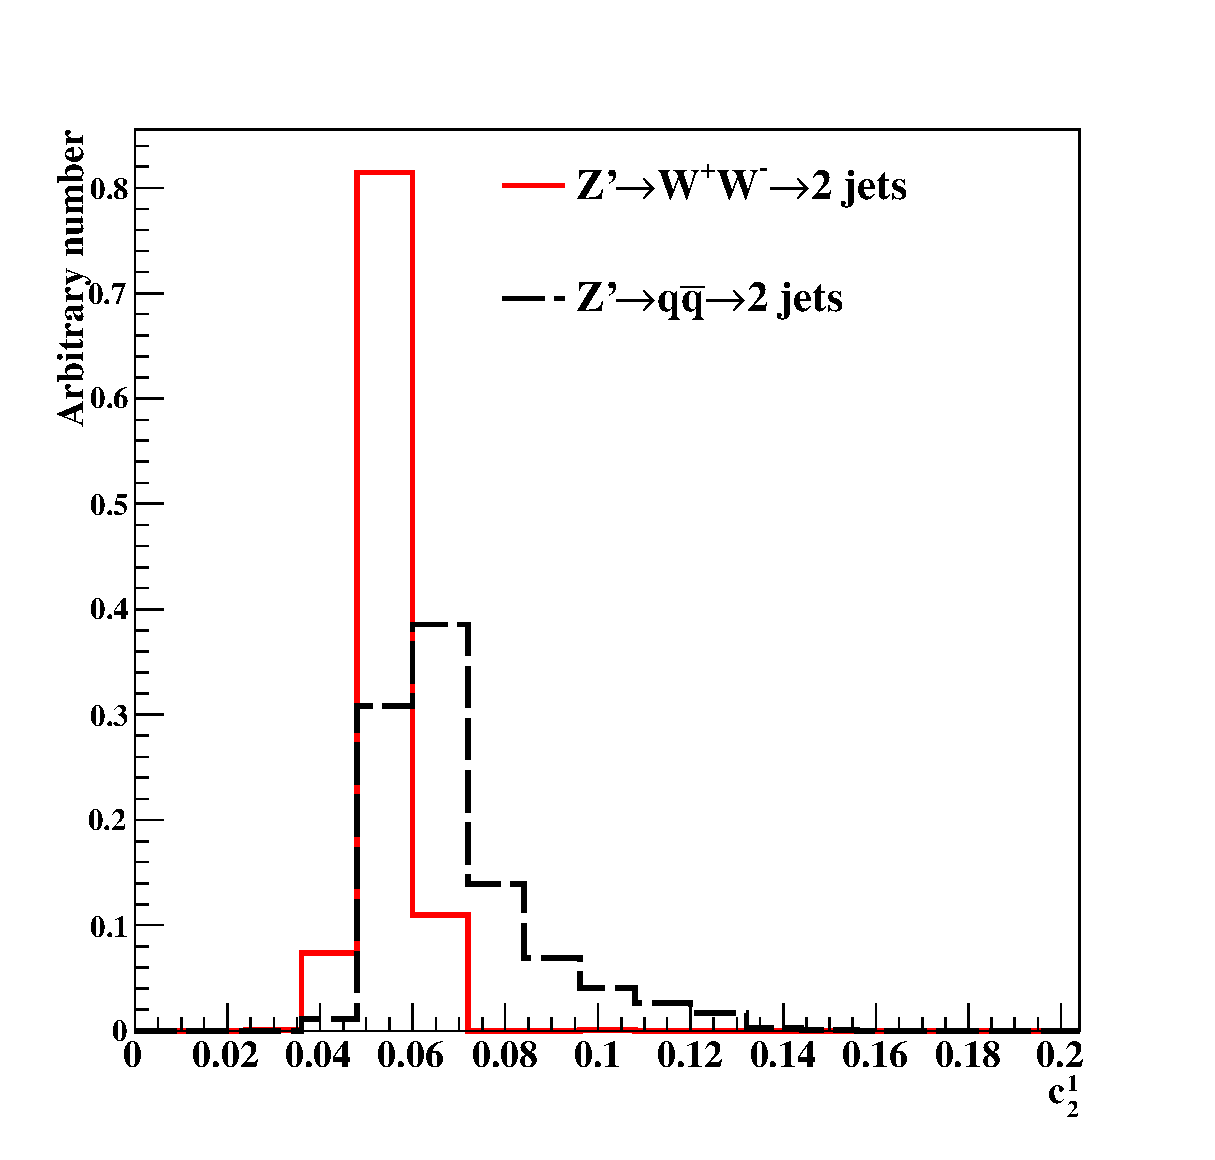
\includegraphics[width=0.3\textwidth]{h_Tau_C/Dis_Rawhit_05GeV_010_c2b1_20tev_04_after_cut_Man_25_no_UOF_new_75pa_for_paper.eps}
   }
   \subfigure[5$\times$5($cm^2$)] {
   \centering
   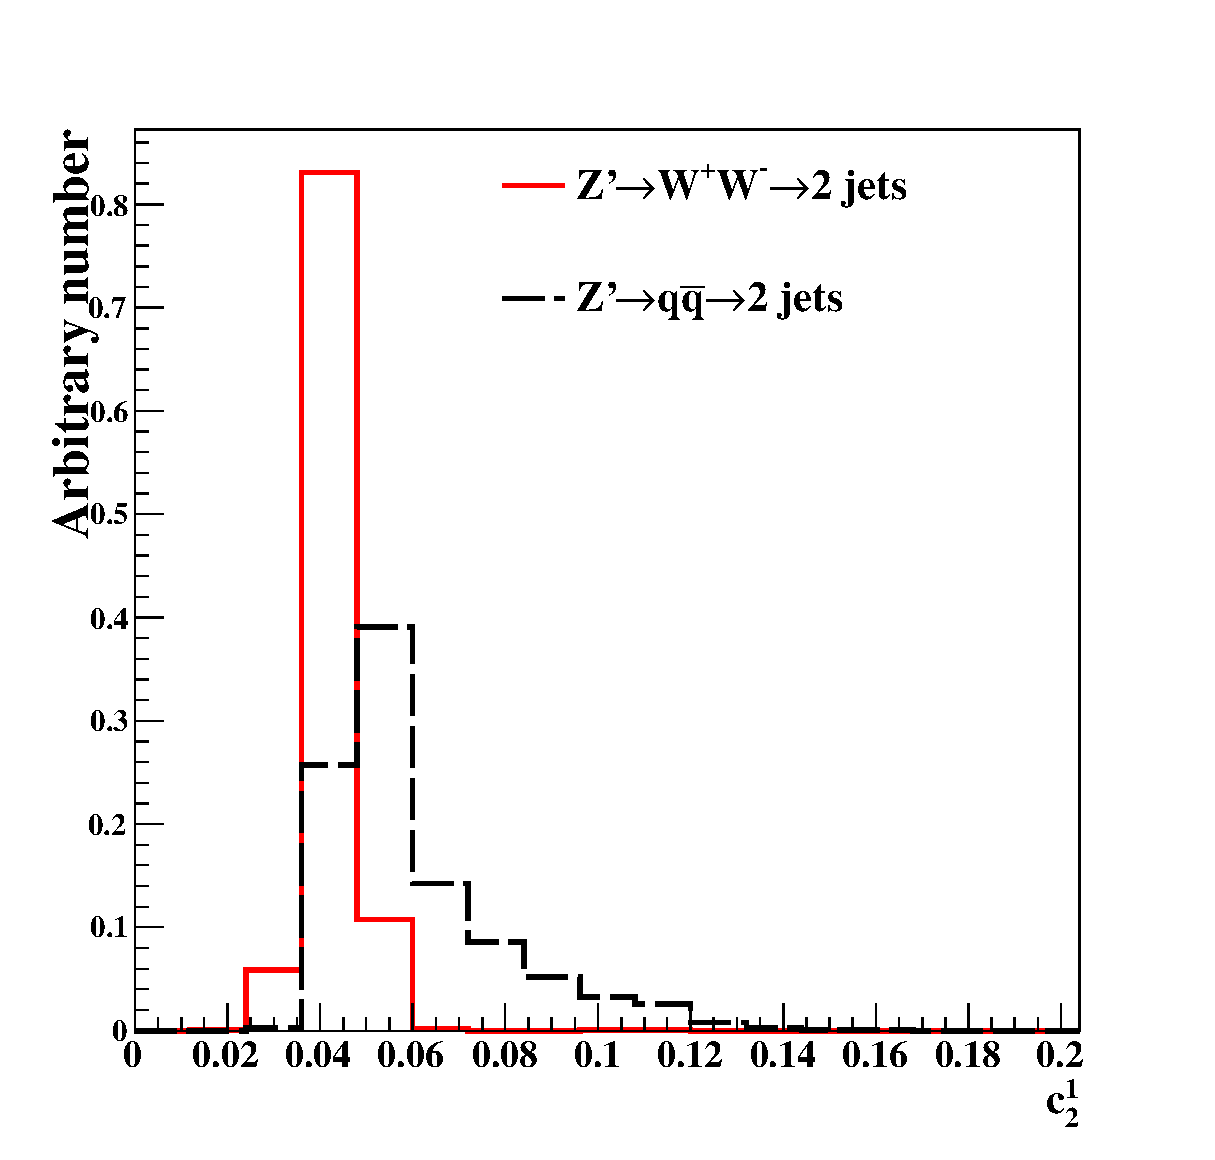
\includegraphics[width=0.3\textwidth]{h_Tau_C/Dis_Rawhit_05GeV_009_c2b1_20tev_04_after_cut_Man_25_no_UOF_new_75pa_for_paper.eps}
   }
   \subfigure[1$\times$1($cm^2$)] {
   \centering
   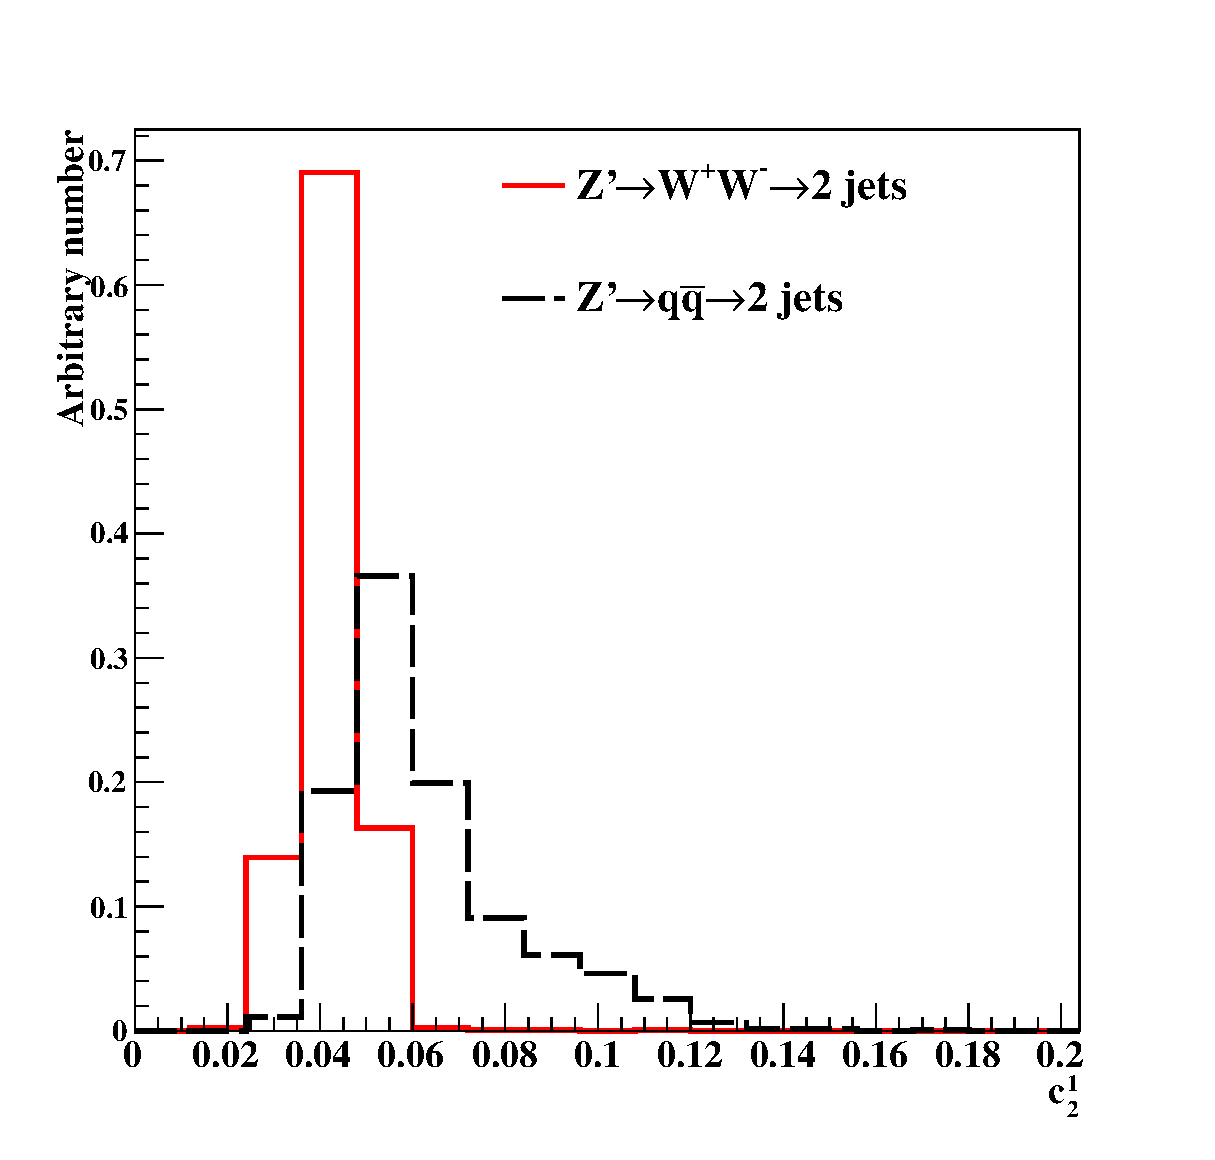
\includegraphics[width=0.3\textwidth]{h_Tau_C/Dis_Rawhit_05GeV_012_c2b1_20tev_04_after_cut_Man_25_no_UOF_new_75pa_for_paper.eps}
   }
\end{center}
\caption{Distributions of Mann-Whitney value U in 20 TeV energy collision for  $C_{2}^{1}$ in different detector sizes. Cell Size in 20$\times$20, 5$\times$5, and 1$\times$1(cm$\times$cm) are shown here.}
\label{fig:Rawhit_05GeV_c2b1_Dis}
\end{figure}

\begin{figure}
\begin{center}
   \subfigure[Z'(5 TeV)] {
   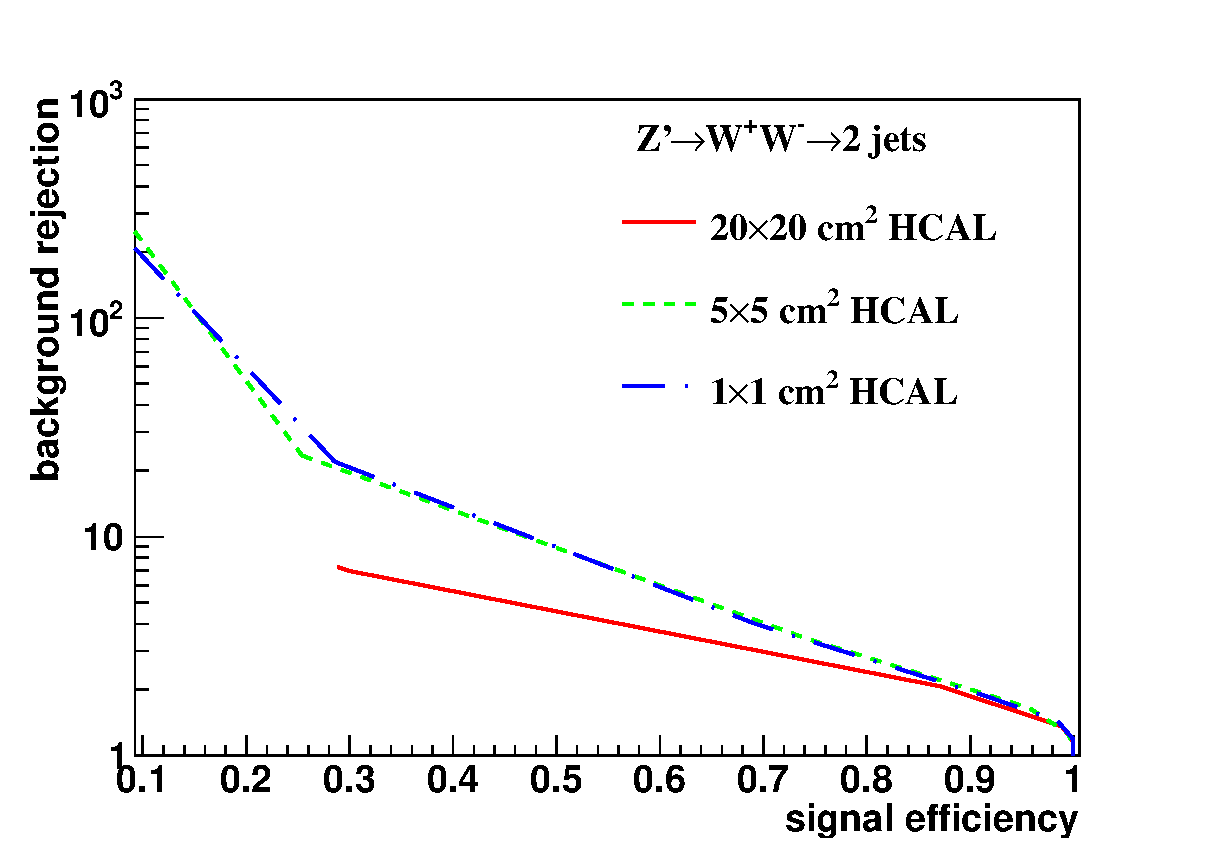
\includegraphics[width=0.43\textwidth]{ROC_Tau_C/Rawhit_05GeV_c2b1_5tev_eff_1_New2_after_cut_25bins_no_UOF_new_75pa.eps}\hfill
   }
   \subfigure[Z'(10 TeV)] {
   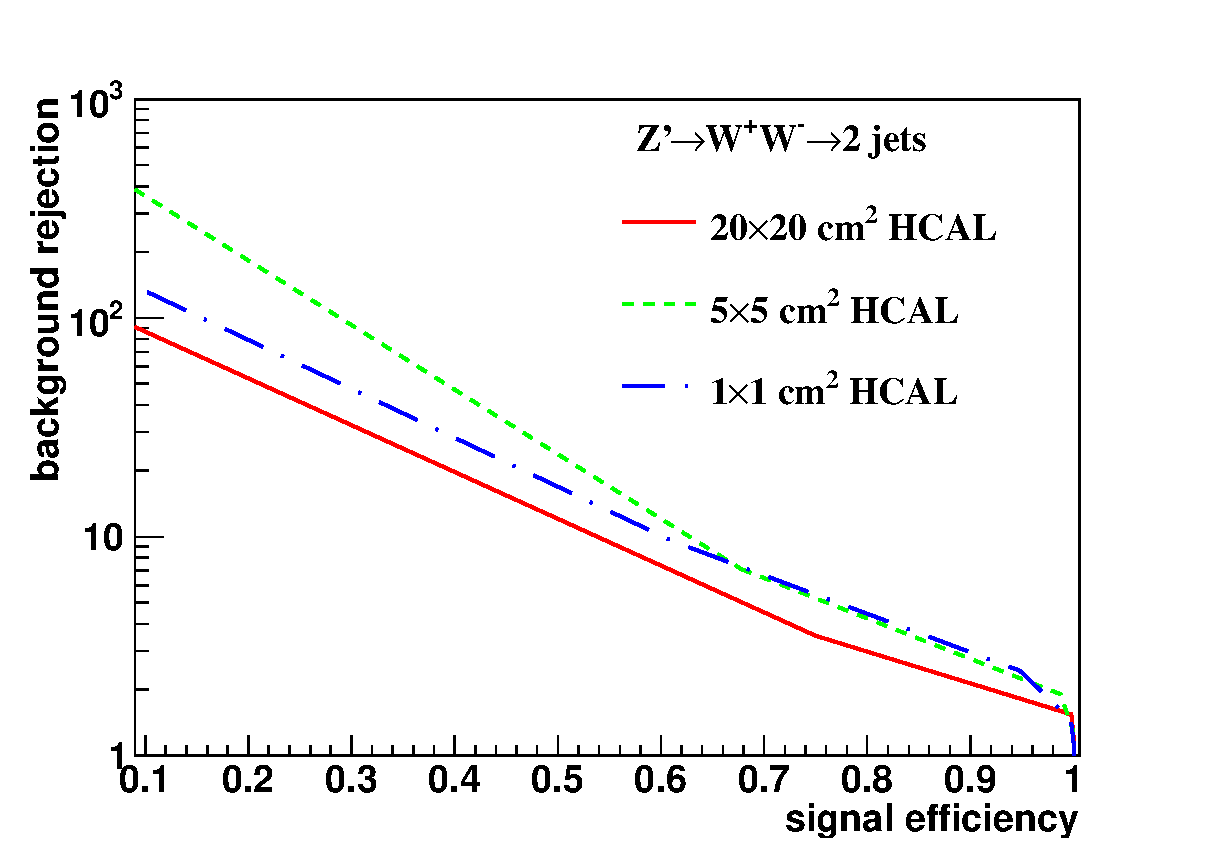
\includegraphics[width=0.43\textwidth]{ROC_Tau_C/Rawhit_05GeV_c2b1_10tev_eff_1_New2_after_cut_25bins_no_UOF_new_75pa.eps}
   }
   \subfigure[Z'(20 TeV)] {
   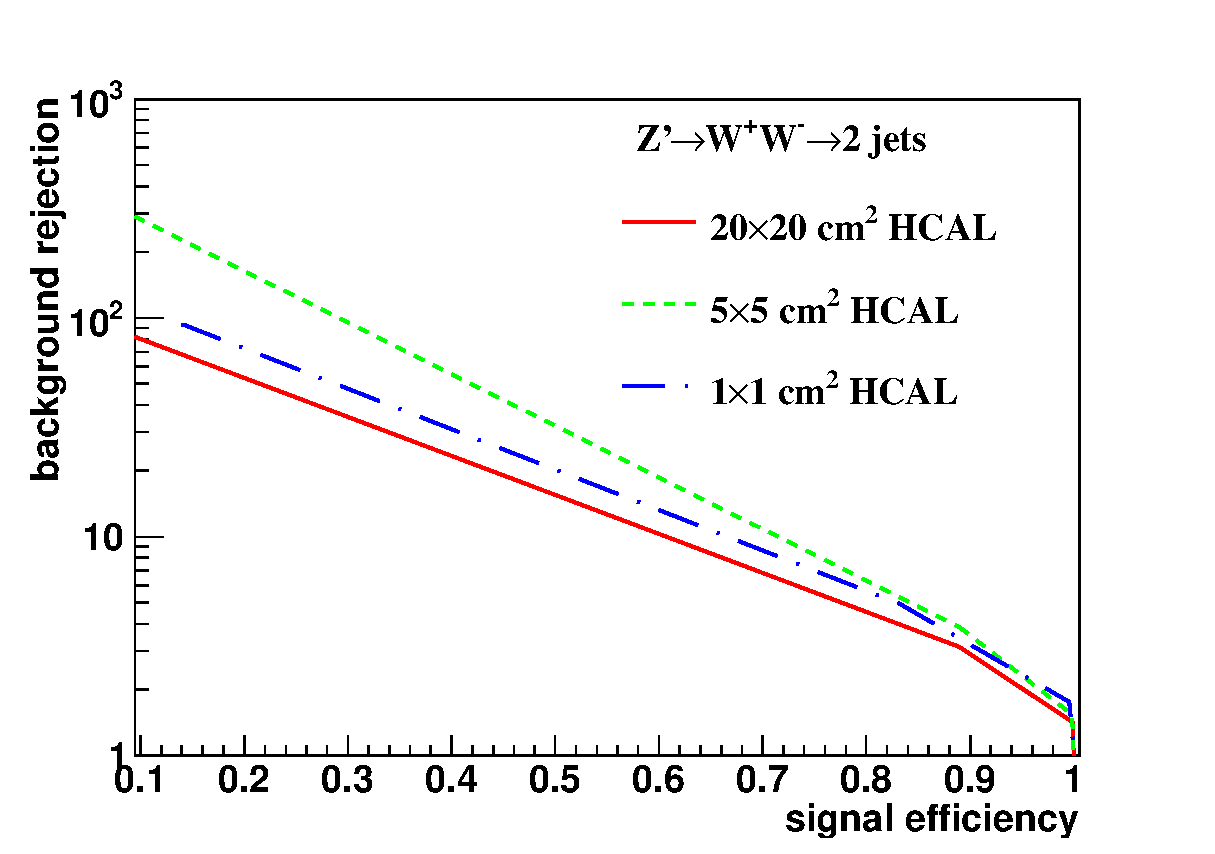
\includegraphics[width=0.43\textwidth]{ROC_Tau_C/Rawhit_05GeV_c2b1_20tev_eff_1_New2_after_cut_25bins_no_UOF_new_75pa.eps}
   }
   \subfigure[Z'(40 TeV)] {
   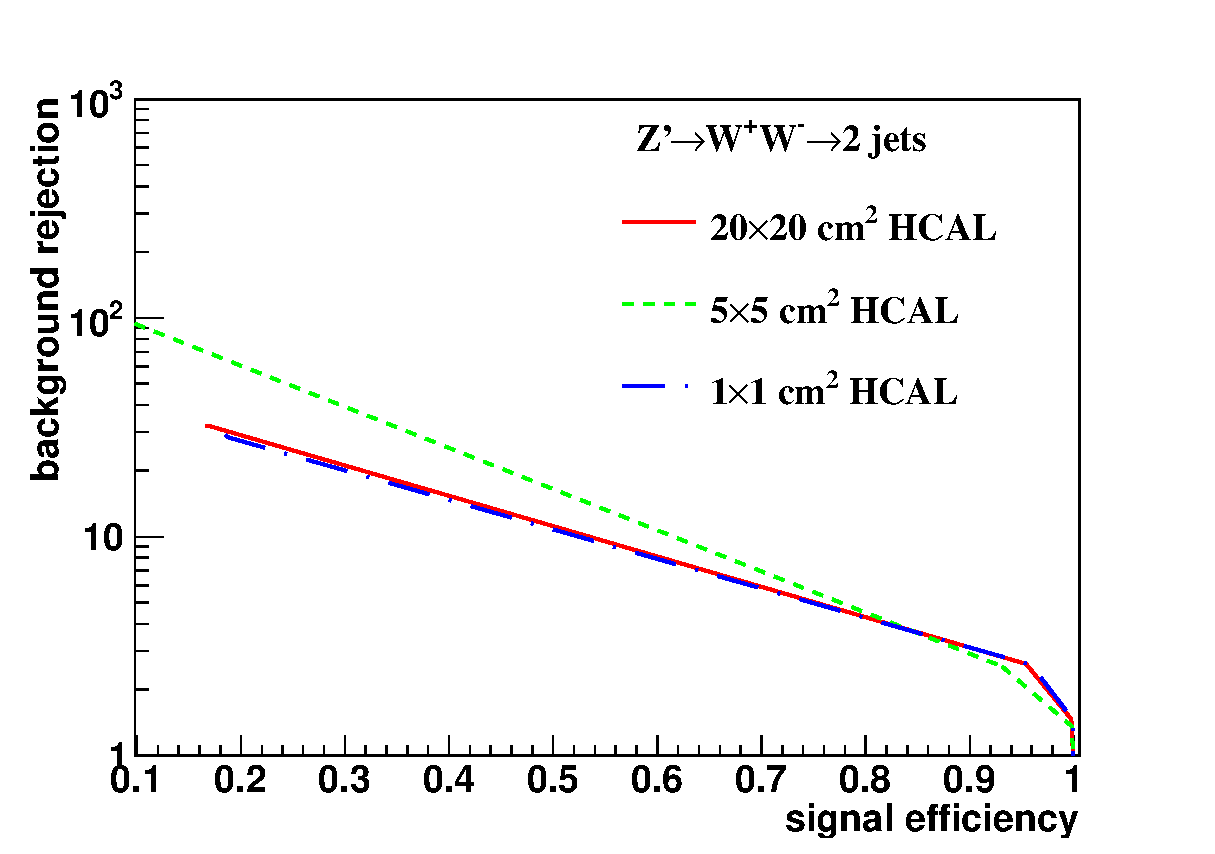
\includegraphics[width=0.43\textwidth]{ROC_Tau_C/Rawhit_05GeV_c2b1_40tev_eff_1_New2_after_cut_25bins_no_UOF_new_75pa.eps}
   }
\end{center}
\caption{Signal efficiency versus background rejection rate using  $C_{2}^{1}$.The energies of collision at (a)5, (b)10, (c)20, (d)40TeV are shown here. In each picture, the three ROC curves correspond to different detector sizes.}
\label{fig:Rawhit_05GeV_c2b1_ROC}
\end{figure}



%25bins
\begin{figure}
\begin{center}
   \subfigure[20$\times$20($cm^2$)] {
   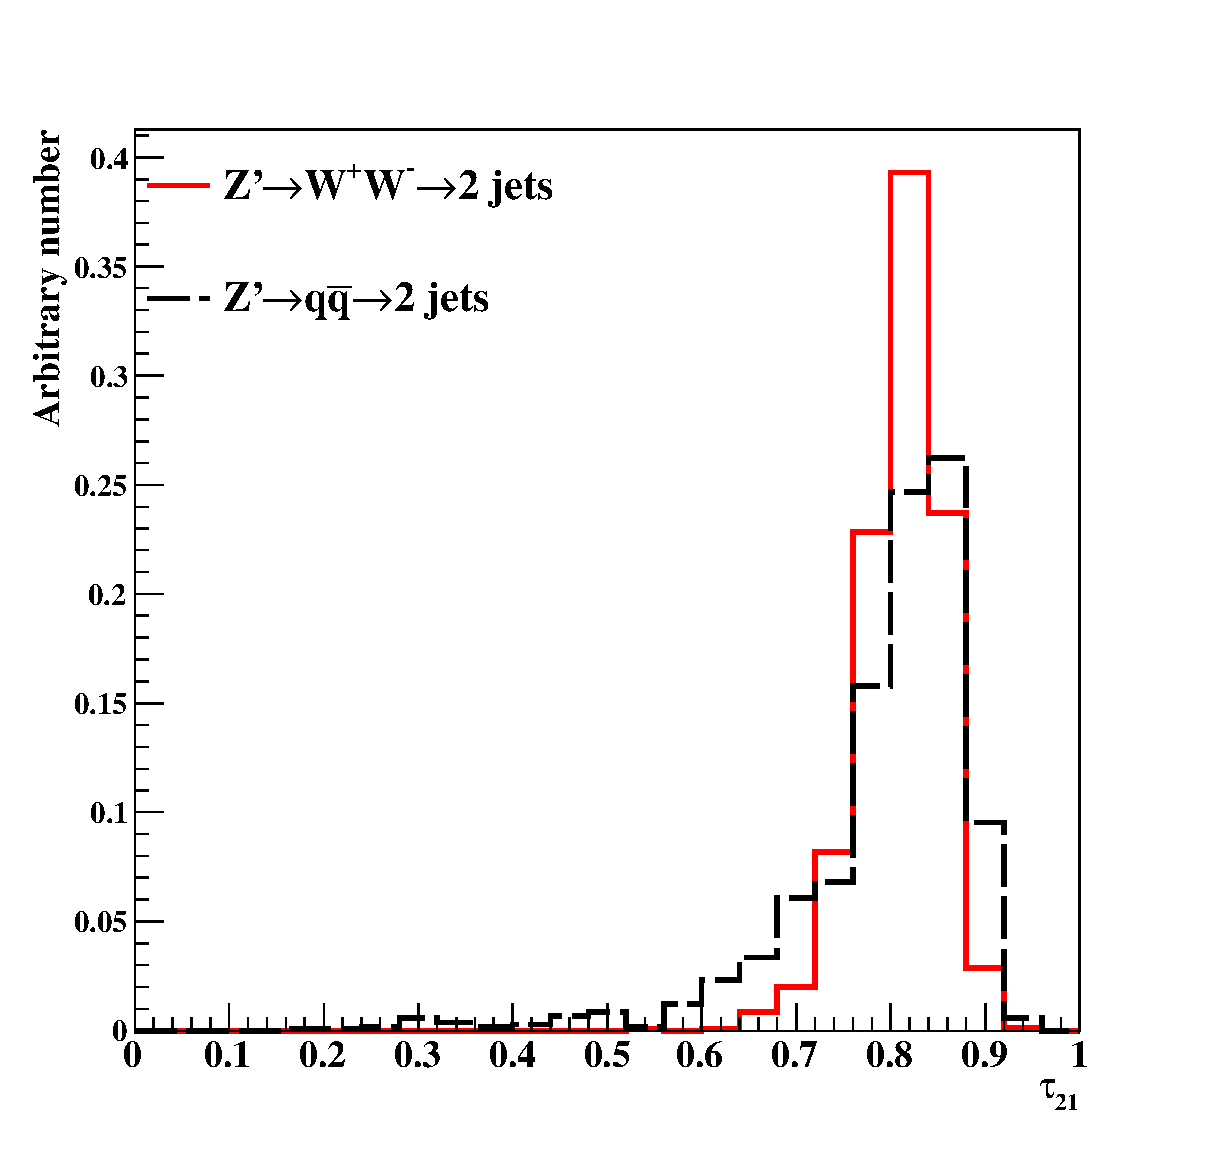
\includegraphics[width=0.3\textwidth]{h_Tau_C/Dis_Rawhit_05GeV_010_tau21_20tev_04_after_cut_Man_25_no_UOF_new_75pa_for_paper.eps}
   }
   \subfigure[5$\times$5($cm^2$)] {
   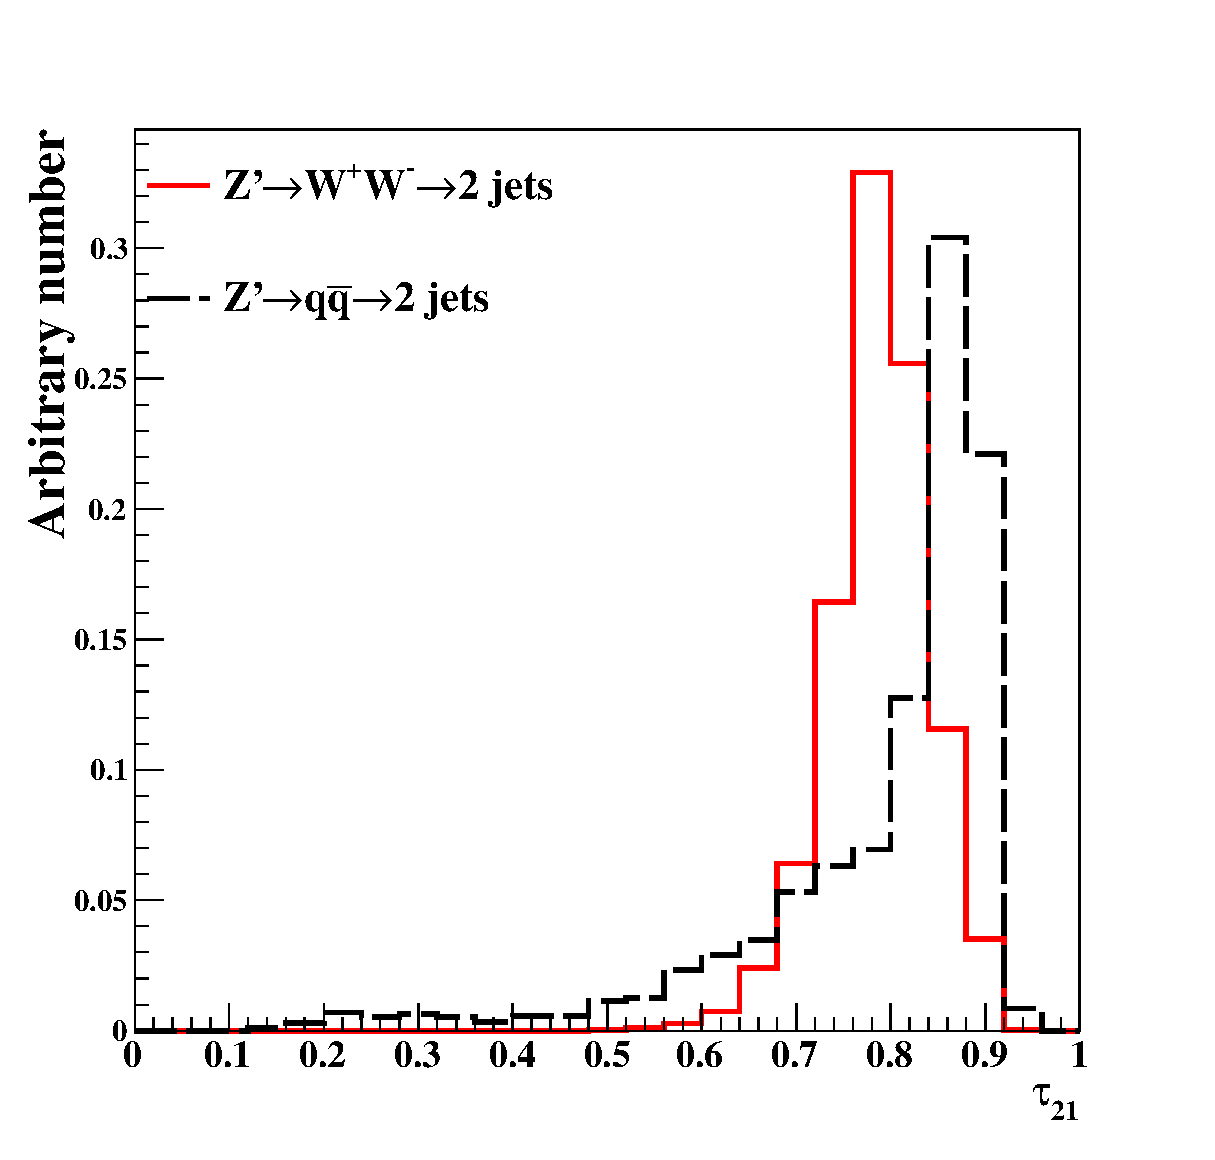
\includegraphics[width=0.3\textwidth]{h_Tau_C/Dis_Rawhit_05GeV_009_tau21_20tev_04_after_cut_Man_25_no_UOF_new_75pa_for_paper.eps}
   }
   \subfigure[1$\times$1($cm^2$)] {
   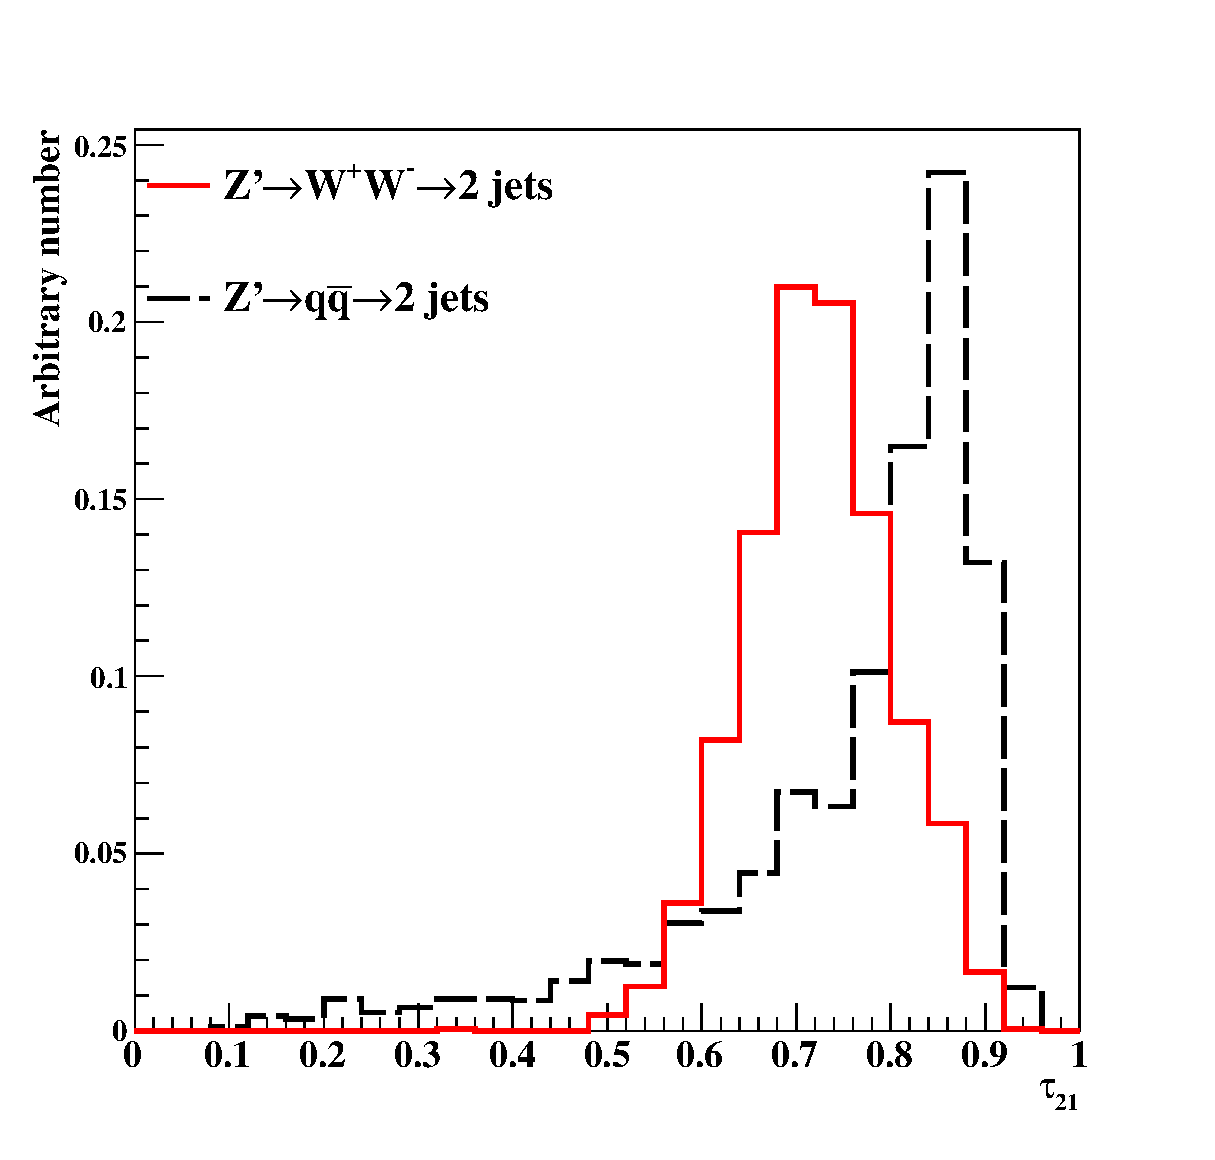
\includegraphics[width=0.3\textwidth]{h_Tau_C/Dis_Rawhit_05GeV_012_tau21_20tev_04_after_cut_Man_25_no_UOF_new_75pa_for_paper.eps}
   }
\end{center}
\caption{Distributions of Mann-Whitney value U in 20 TeV energy collision for $\tau_{21}$  in different detector sizes. Cell Size in 20$\times$20, 5$\times$5, and 1$\times$1(cm$\times$cm) are shown here.}
\label{fig:Rawhit_05GeV_tau21_Dis}
\end{figure}

\begin{figure}
\begin{center}
   \subfigure[Z'(5 TeV)] {
   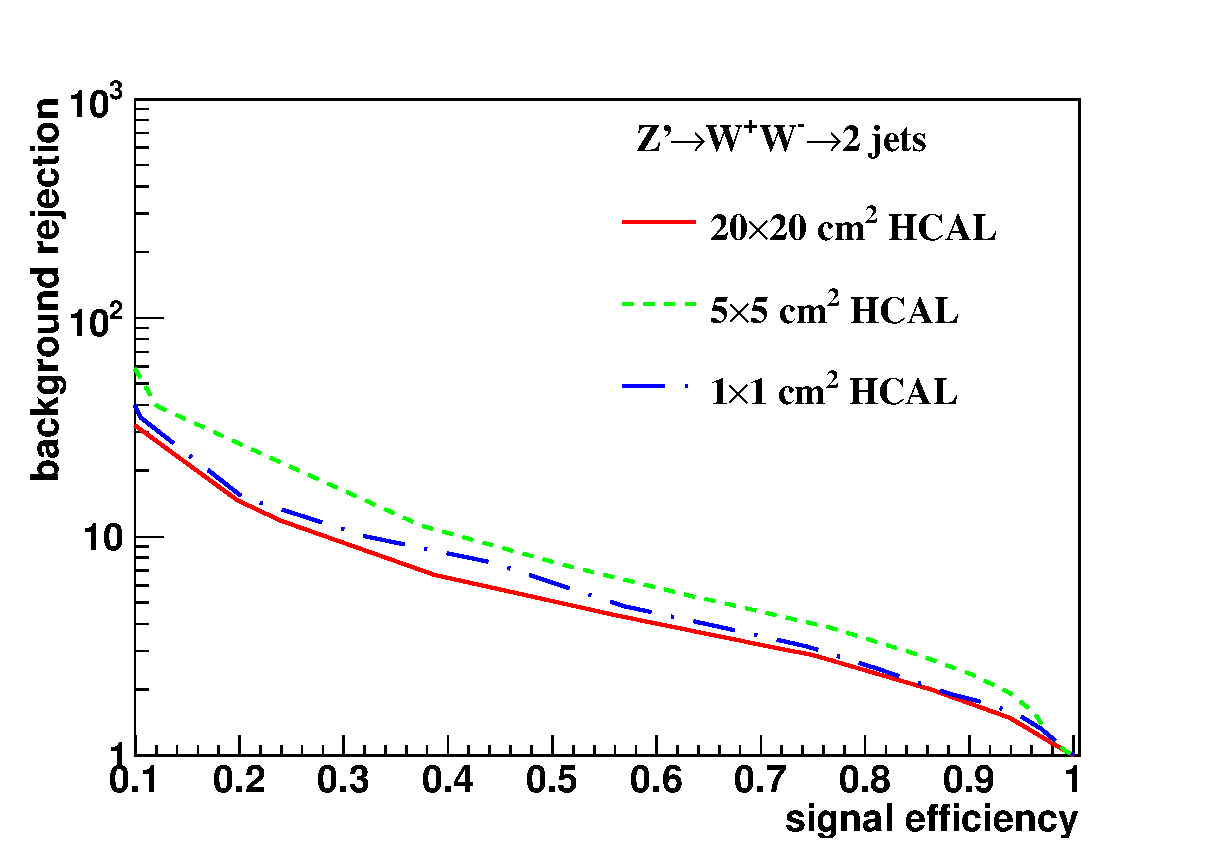
\includegraphics[width=0.43\textwidth]{ROC_Tau_C/Rawhit_05GeV_tau21_5tev_eff_1_New2_after_cut_25bins_no_UOF_new_75pa.eps}\hfill
   }
   \subfigure[Z'(10 TeV)] {
   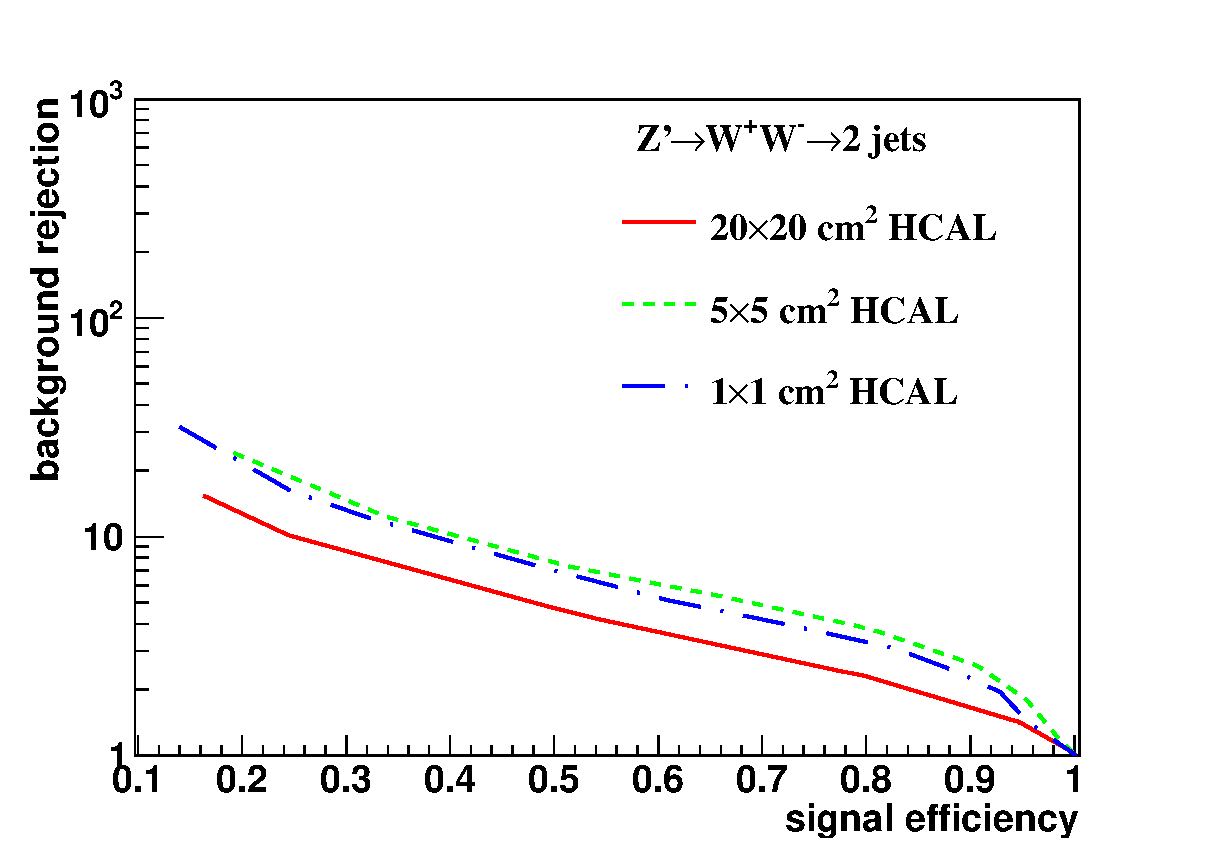
\includegraphics[width=0.43\textwidth]{ROC_Tau_C/Rawhit_05GeV_tau21_10tev_eff_1_New2_after_cut_25bins_no_UOF_new_75pa.eps}
   }
   \subfigure[Z'(20 TeV)] {
   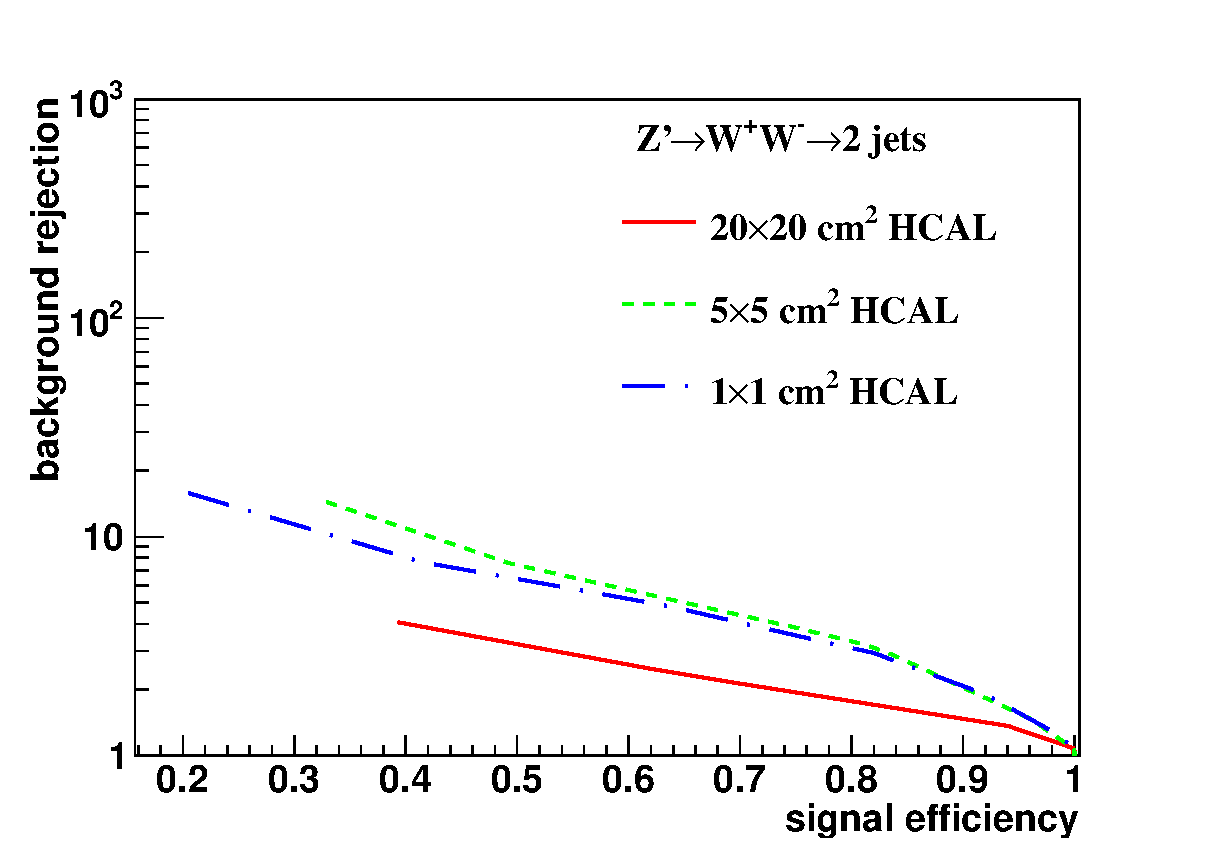
\includegraphics[width=0.43\textwidth]{ROC_Tau_C/Rawhit_05GeV_tau21_20tev_eff_1_New2_after_cut_25bins_no_UOF_new_75pa.eps}
   }
   \subfigure[Z'(40 TeV)] {
   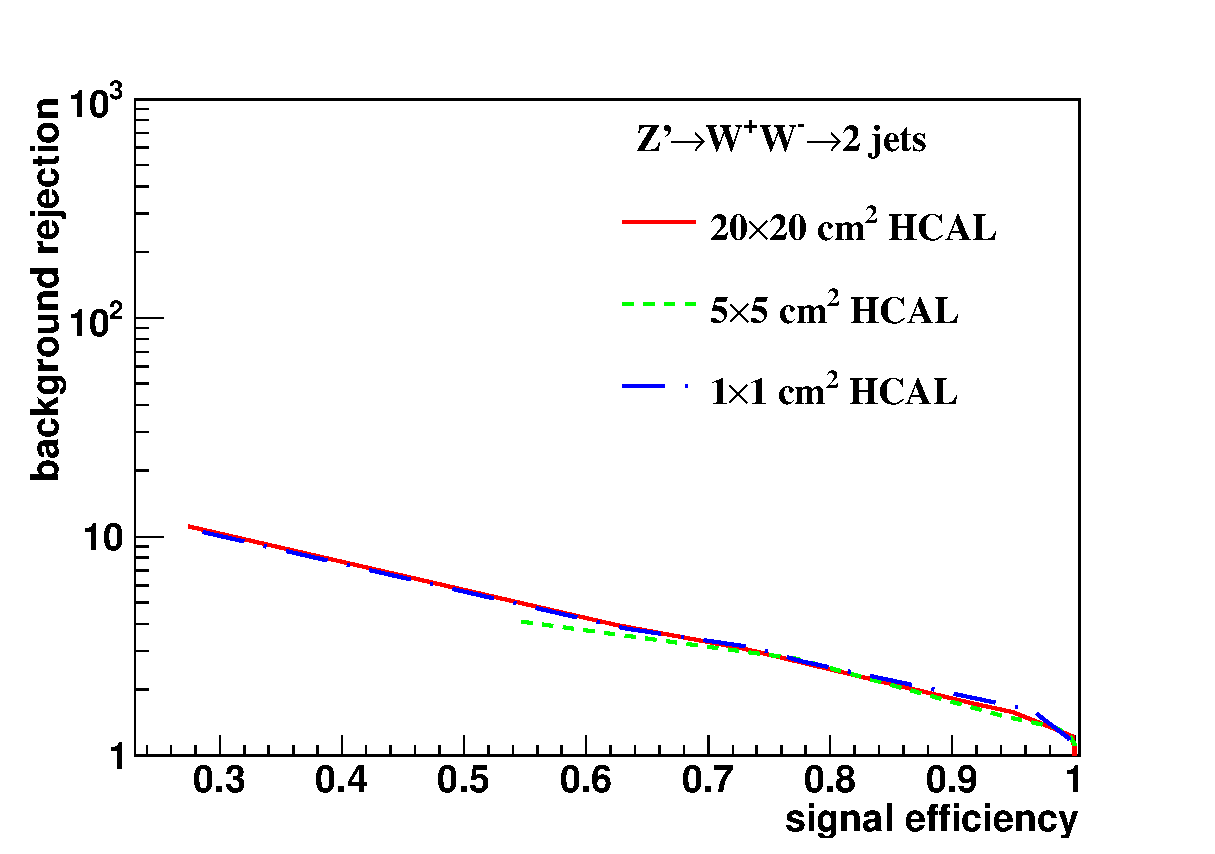
\includegraphics[width=0.43\textwidth]{ROC_Tau_C/Rawhit_05GeV_tau21_40tev_eff_1_New2_after_cut_25bins_no_UOF_new_75pa.eps}
   }
\end{center}
\caption{Signal efficiency versus background rejection rate using $\tau_{21}$.The energies of collision at (a)5, (b)10, (c)20, (d)40TeV are shown here. In each picture, the three ROC curves correspond to different detector sizes.}
\label{fig:Rawhit_05GeV_tau21_ROC}
\end{figure}




%25bins
\begin{figure}
\begin{center}
   \subfigure[20$\times$20($cm^2$)] {
   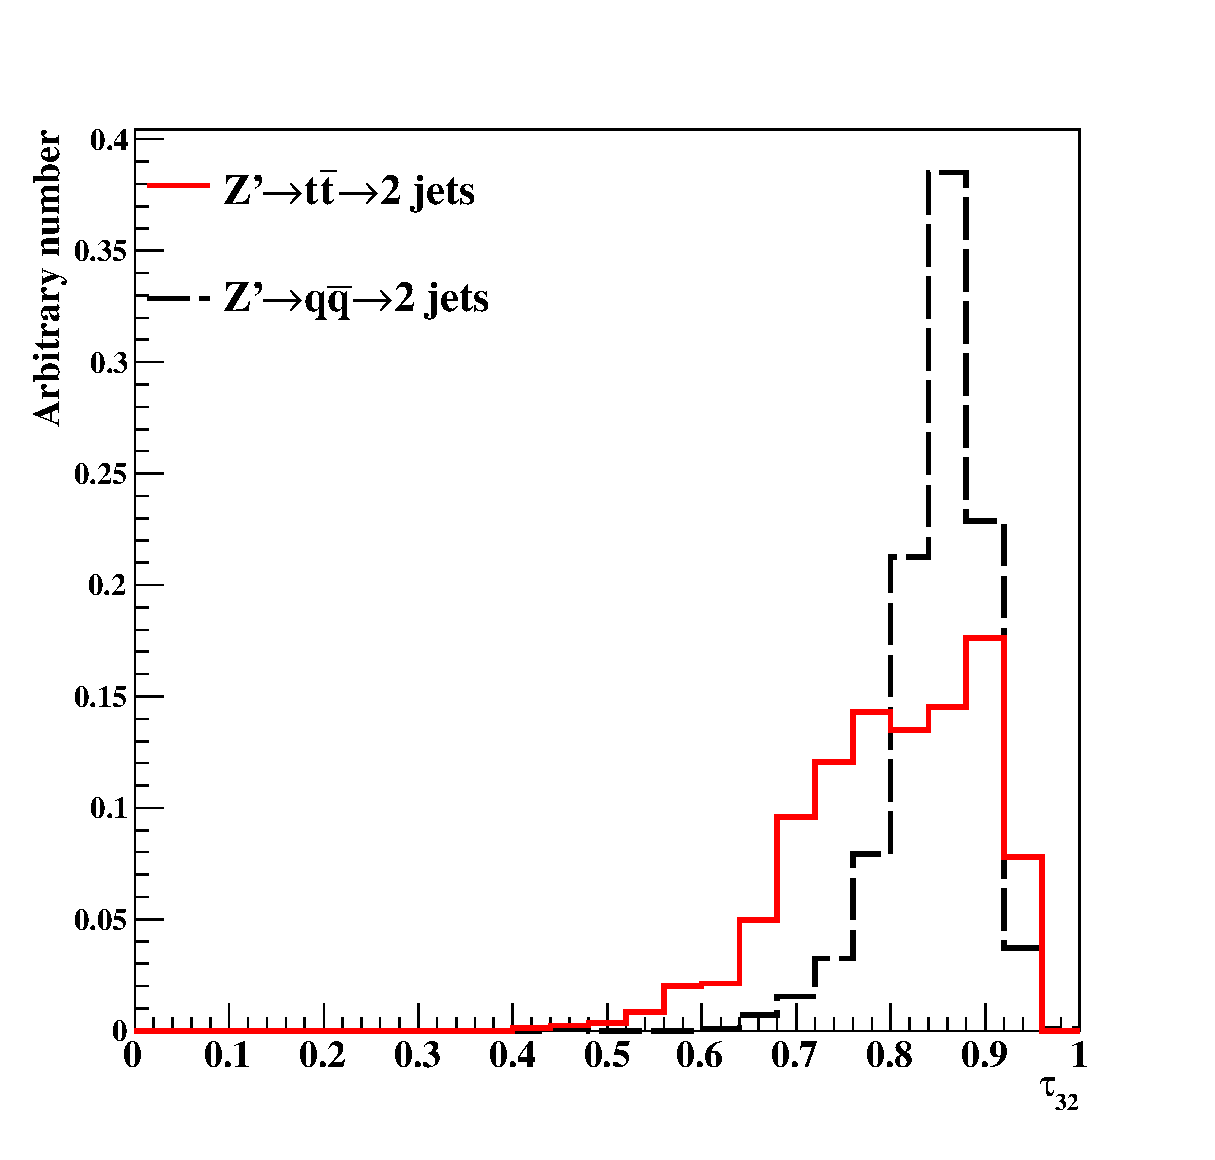
\includegraphics[width=0.3\textwidth]{h_Tau_C/Dis_Rawhit_05GeV_010_tau32_20tev_04_after_cut_Man_25_no_UOF_new_75pa_for_paper.eps}
   }
   \subfigure[5$\times$5($cm^2$)] {
   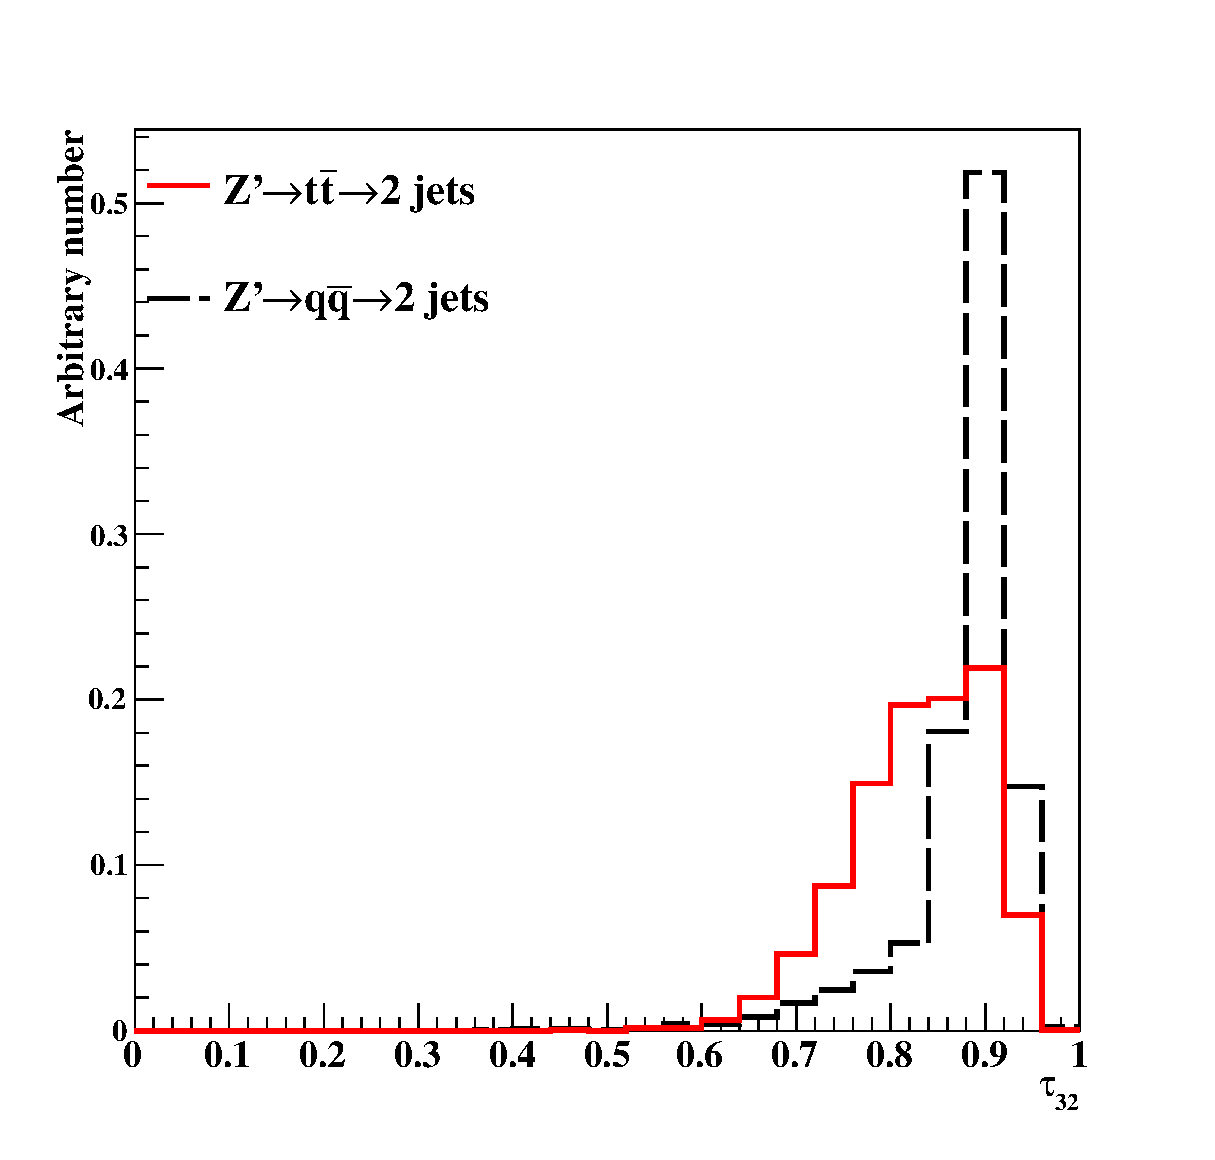
\includegraphics[width=0.3\textwidth]{h_Tau_C/Dis_Rawhit_05GeV_009_tau32_20tev_04_after_cut_Man_25_no_UOF_new_75pa_for_paper.eps}
   }
   \subfigure[1$\times$1($cm^2$)] {
   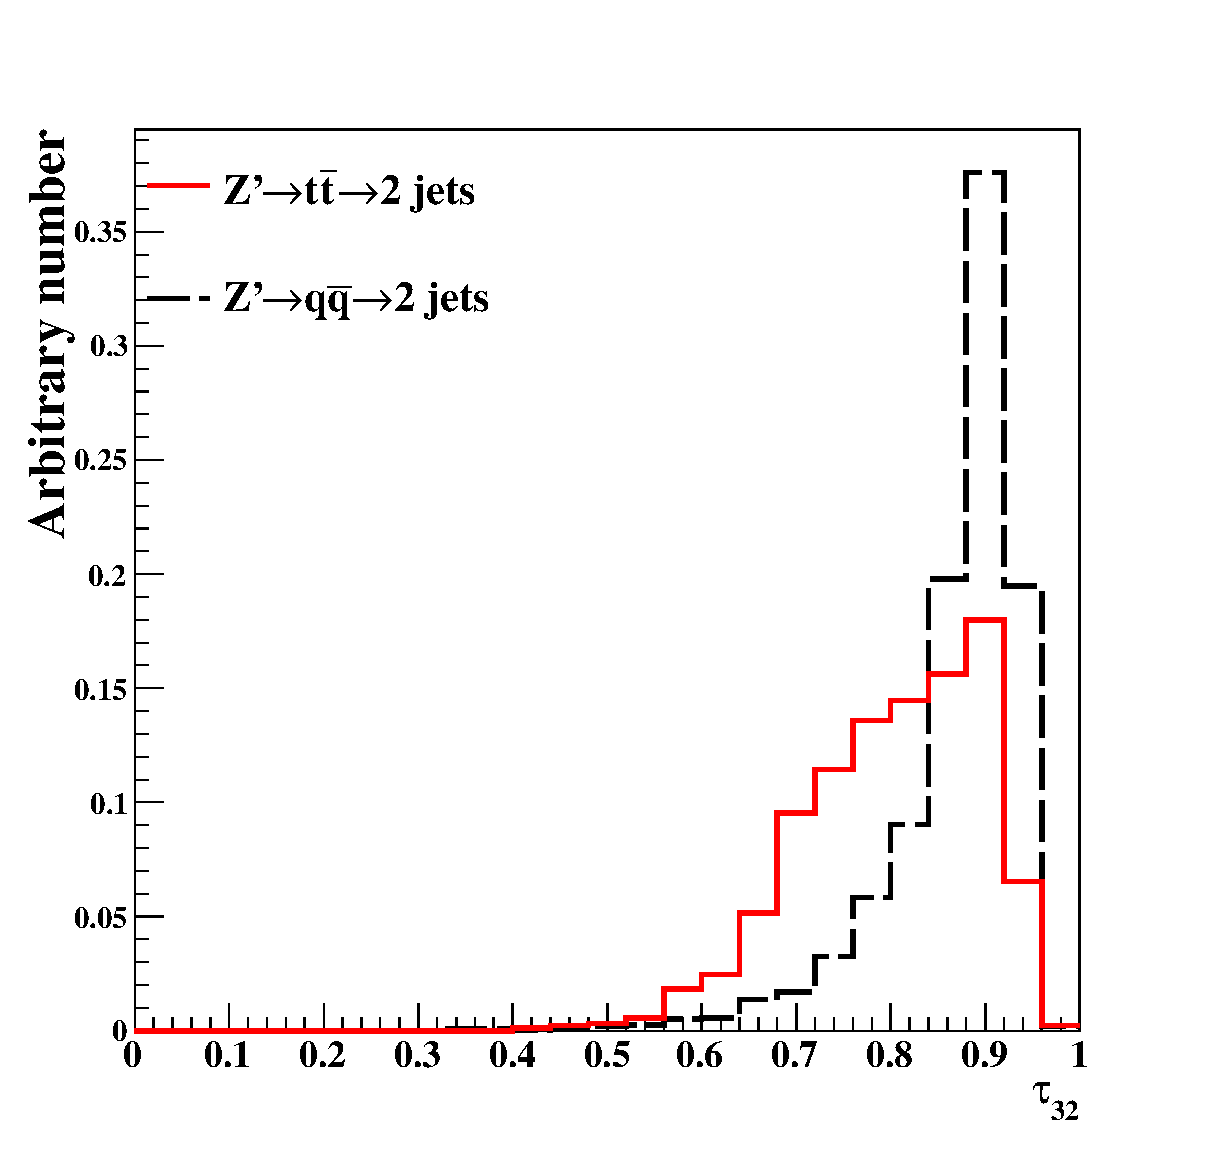
\includegraphics[width=0.3\textwidth]{h_Tau_C/Dis_Rawhit_05GeV_012_tau32_20tev_04_after_cut_Man_25_no_UOF_new_75pa_for_paper.eps}
   }
\end{center}
\caption{Distributions of Mann-Whitney value U in 20 TeV energy collision for $\tau_{32}$  in different detector sizes. Cell Size in 20$\times$20, 5$\times$5, and 1$\times$1(cm$\times$cm) are shown here.}
\label{fig:Rawhit_05GeV_tau32_Dis}
\end{figure}

\begin{figure}
\begin{center}
   \subfigure[Z'(5 TeV)] {
   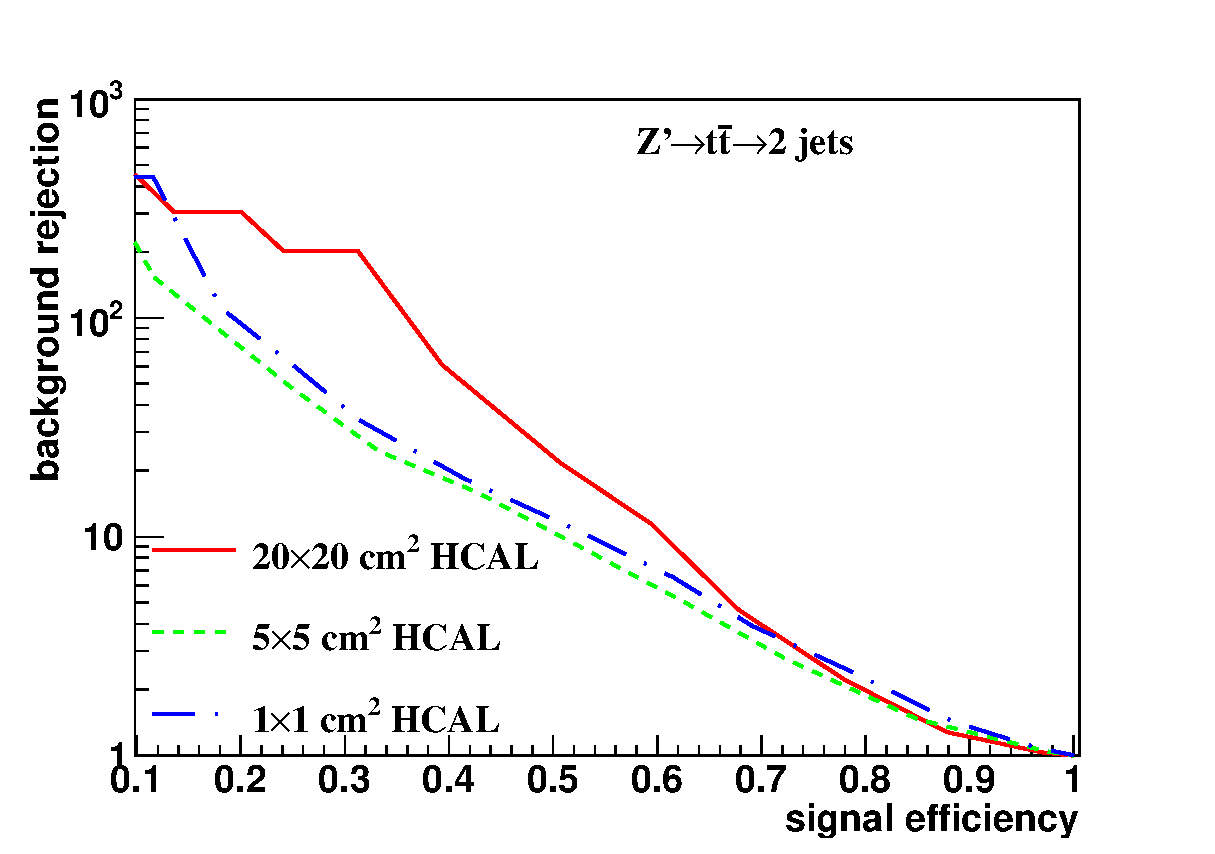
\includegraphics[width=0.43\textwidth]{ROC_Tau_C/Rawhit_05GeV_tau32_5tev_eff_1_New2_after_cut_25bins_no_UOF_new_75pa.eps}\hfill
   }
   \subfigure[Z'(10 TeV)] {
   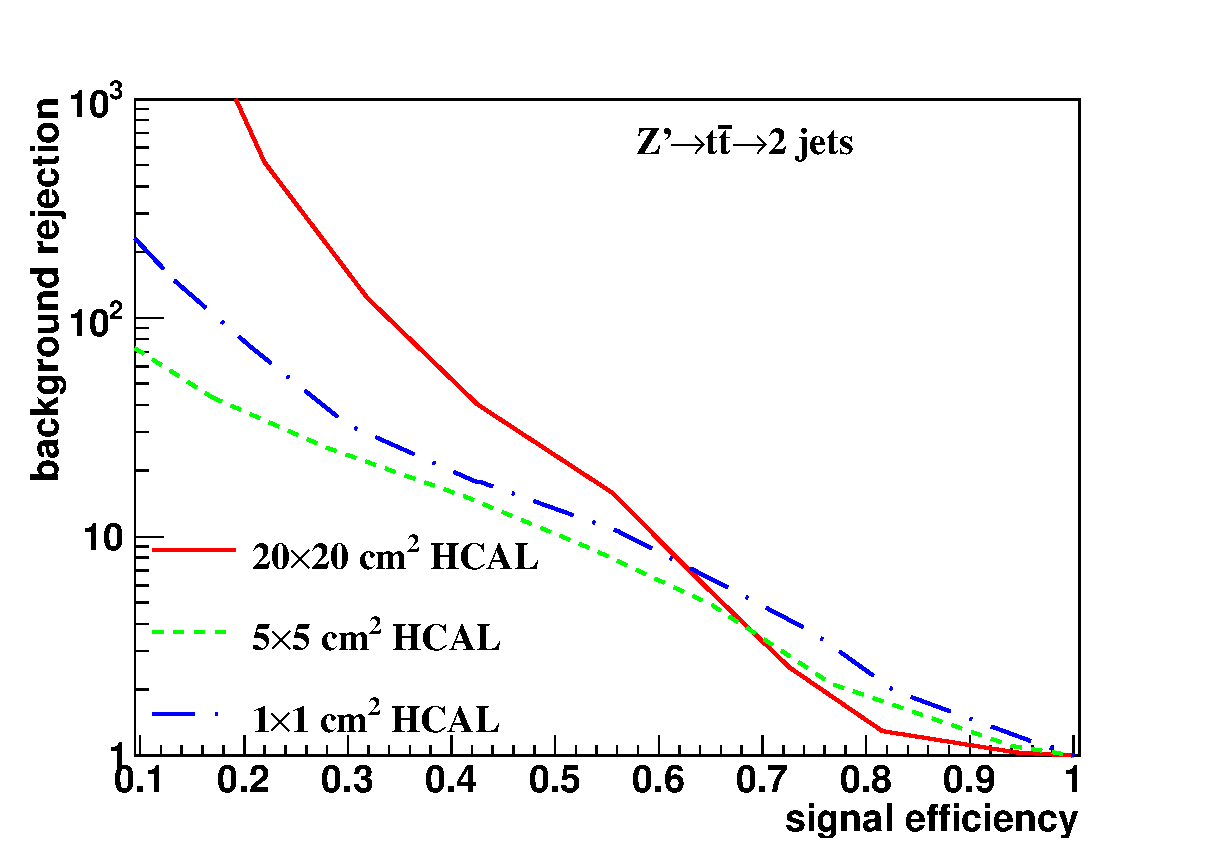
\includegraphics[width=0.43\textwidth]{ROC_Tau_C/Rawhit_05GeV_tau32_10tev_eff_1_New2_after_cut_25bins_no_UOF_new_75pa.eps}
   }
   \subfigure[Z'(20 TeV)] {
   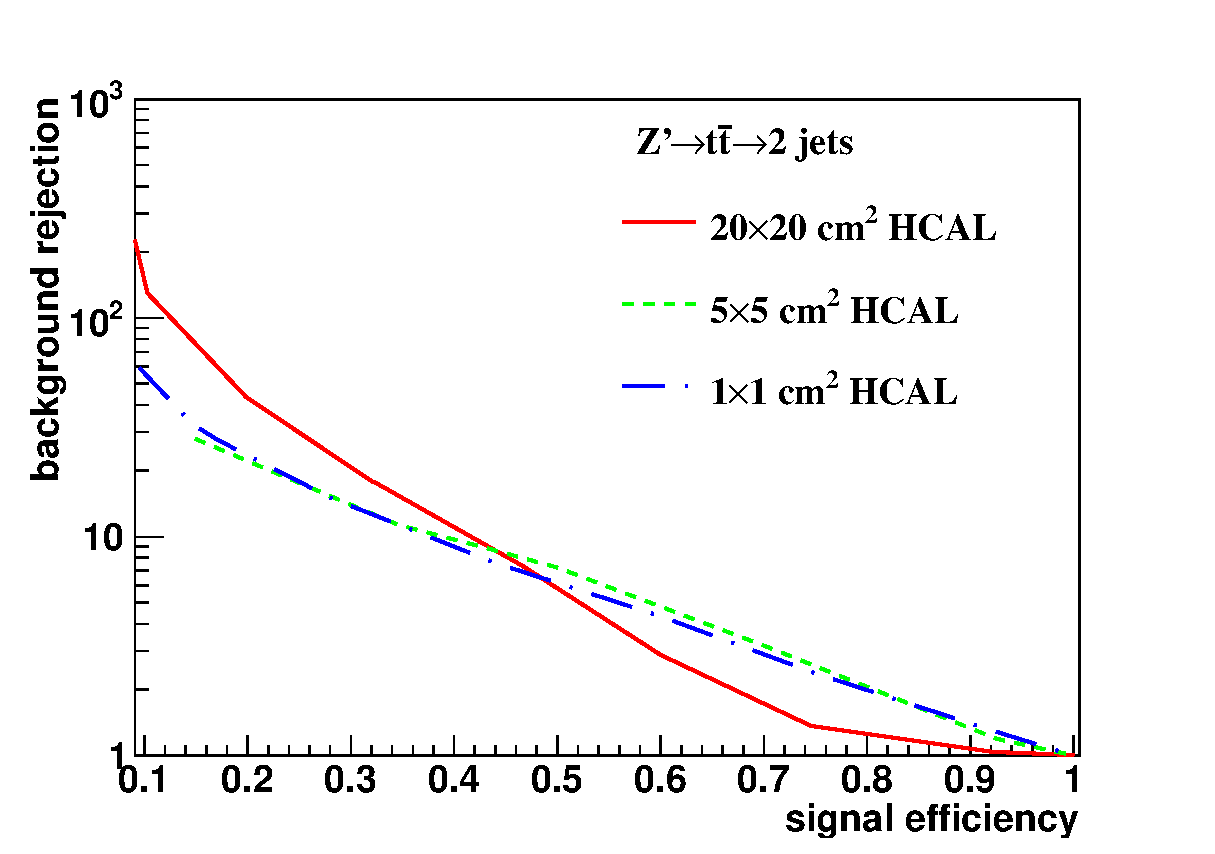
\includegraphics[width=0.43\textwidth]{ROC_Tau_C/Rawhit_05GeV_tau32_20tev_eff_1_New2_after_cut_25bins_no_UOF_new_75pa.eps}
   }
   \subfigure[Z'(40 TeV)] {
   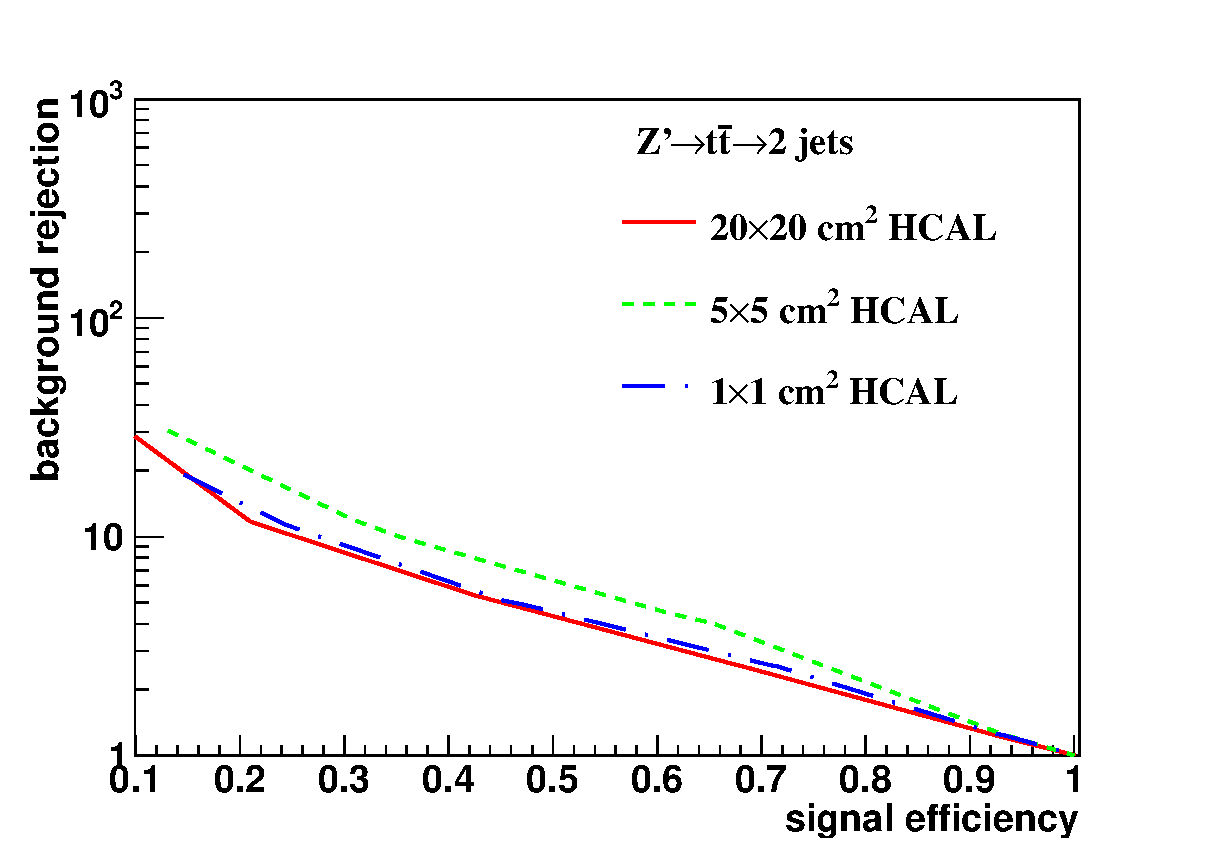
\includegraphics[width=0.43\textwidth]{ROC_Tau_C/Rawhit_05GeV_tau32_40tev_eff_1_New2_after_cut_25bins_no_UOF_new_75pa.eps}
   }
\end{center}
\caption{Signal efficiency versus background rejection rate using $\tau_{32}$.The energies of collision at (a)5, (b)10, (c)20, (d)40TeV are shown here. In each picture, the three ROC curves correspond to different detector sizes.}
\label{fig:Rawhit_05GeV_tau32_ROC}
\end{figure}

%25bins
\begin{figure}
\begin{center}
   \subfigure[$\tau_{21}$] {
   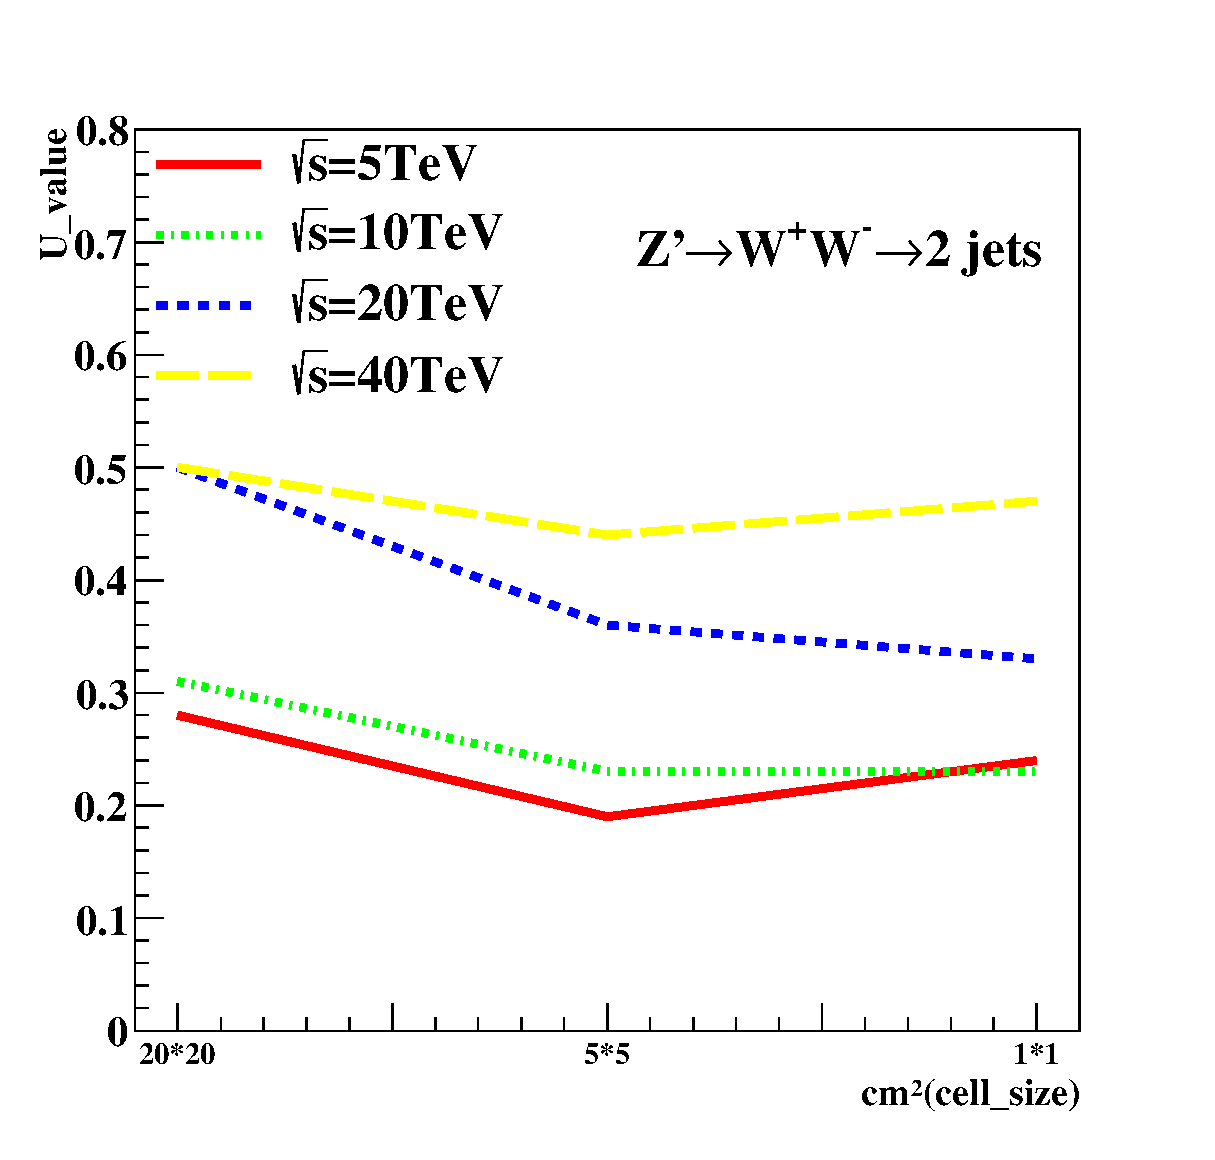
\includegraphics[width=0.3\textwidth]{Mann_Sum/raw_05_tau21_summary_U_after_cut_25bins_no_UOF_new_75pa.eps}\hfill
   }
   \subfigure[$\tau_{32}$ ] {
   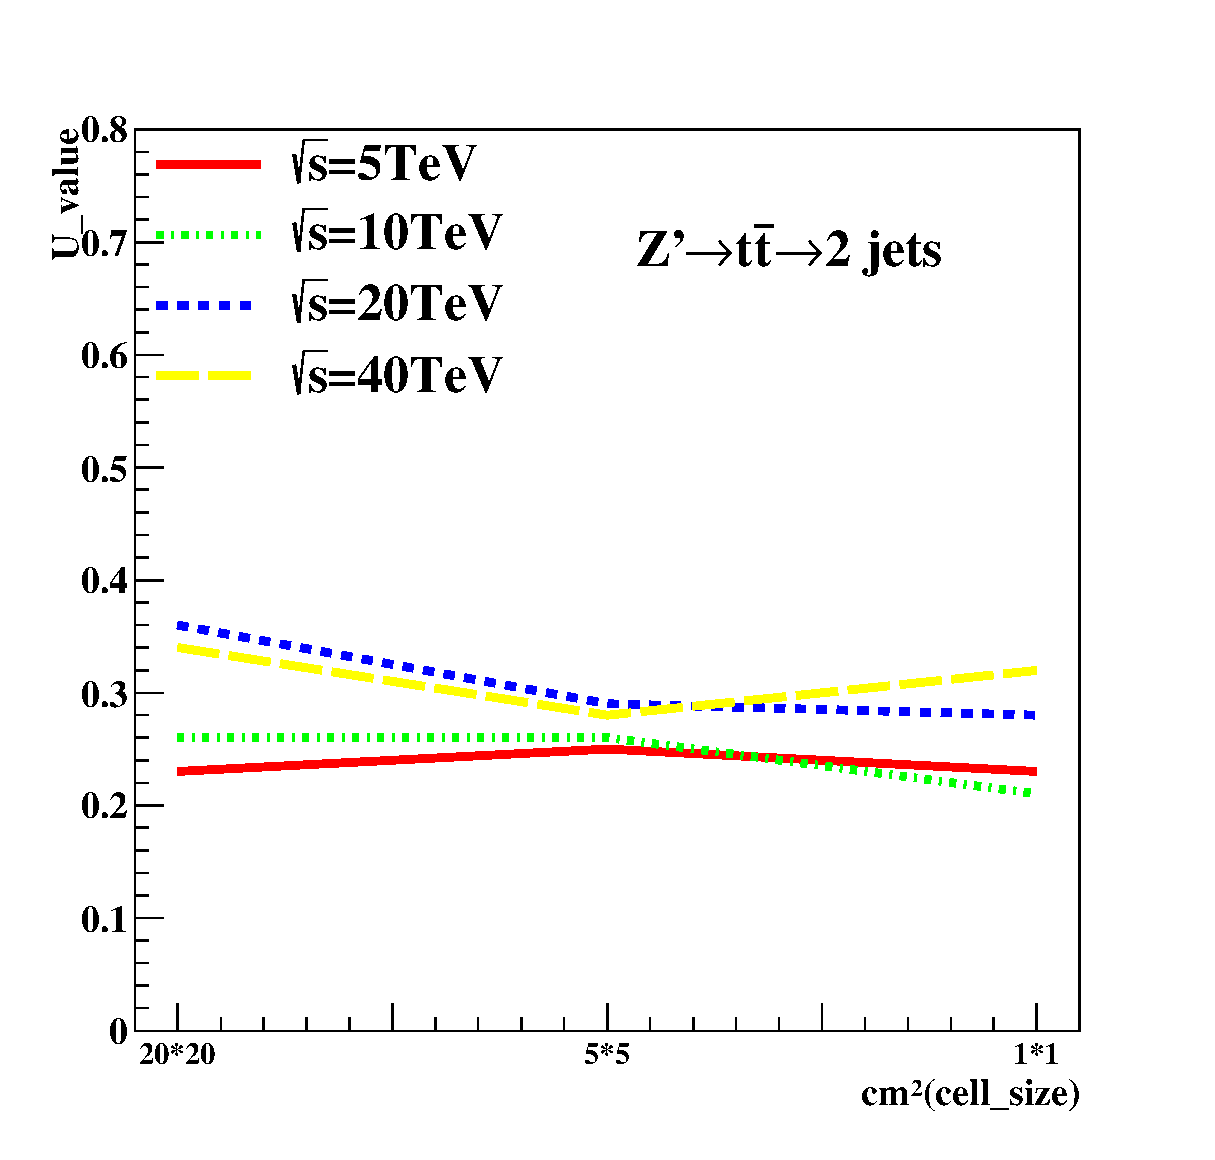
\includegraphics[width=0.3\textwidth]{Mann_Sum/raw_05_tau32_summary_U_after_cut_25bins_no_UOF_new_75pa.eps}
   }
   \subfigure[$c_2^{(1)}$] {
   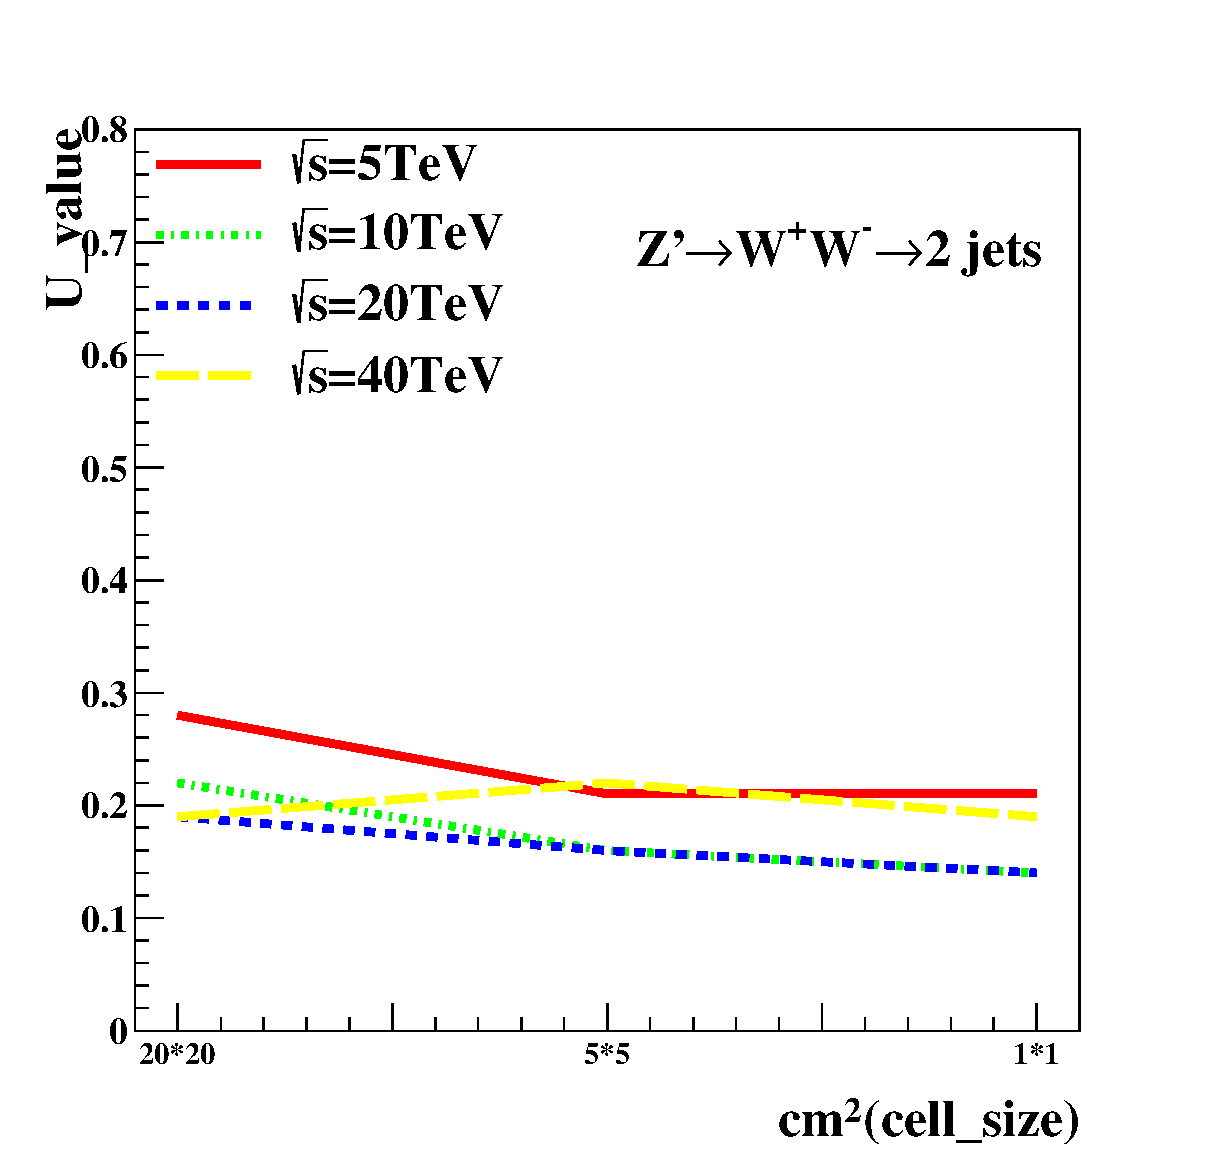
\includegraphics[width=0.3\textwidth]{Mann_Sum/raw_05_c2b1_summary_U_after_cut_25bins_no_UOF_new_75pa.eps}
   }
   \end{center}
\caption{The Mann-Whitney U values for $\tau_{21}$,$\tau_{32}$ and $c_2^{(1)}$ reconstructed from calorimeter hit at 05GeV cut with different collision energies correspond to different detector sizes in rawhit cut with 05GeV. The energies of collision at 5, 10, 20, 40, 20, 40TeV are shown in each figure.}
\label{fig:Rawhit_05GeV_total_Mann}
\end{figure}



